% \documentclass[twoside]{uva-inf-bachelor-thesis}
\documentclass{uva-inf-bachelor-thesis}
%\usepackage[dutch]{babel}

% \usepackage[demo]{graphicx}
\usepackage{float}
\usepackage[backend=biber, style=numeric-comp, sorting=none]{biblatex}
\addbibresource{references.bib}
\usepackage[utf8]{inputenc}
\usepackage[T1]{fontenc}

\usepackage{xcolor}
\usepackage{afterpage}
\usepackage[toc,page]{appendix}

\usepackage{relsize}
\usepackage{moresize}

\usepackage{graphicx}
\usepackage{geometry}

% [CHANGE] The title of your thesis. If your thesis has a subtitle, then this
% should appear right below the main title, in a smaller font.
% \newcommand{\theTitle}{The first sentence \\
% \vspace{0.5em}
% the second sentence}
% \newcommand{\theSubTitle}{a smaller subtitle}


% % [CHANGE] Your full name. In case of multiple names, you can include their
% % initials as well, e.g. "Robin G.J. van Achteren".
% \newcommand{\theAuthor}{Lex Bolt}

% % [CHANGE] Your student ID, as this has been assigned to you by the UvA
% % administration.
% \newcommand{\theStudentID}{13335022}

% % [CHANGE] The name of your supervisor(s). Include the titles of your supervisor(s),
% % as well as the initials for *all* of his/her first names.
% \newcommand{\theSupervisor}{Dr. A. Visser} % Dr. Ing. L. Dorst

% % [CHANGE] The address of the institute at which your supervisor is working.
% % Be sure to include (1) institute (is appropriate), (2) faculty (if
% % appropriate), (3) organisation name, (4) organisation address (2 lines).
% \newcommand{\theInstitute}{
% % Institute for Logic, Language and Computation  
% Informatics Institute \\
% Faculty of Science\\
% University of Amsterdam\\
% Science Park 904 \\ % Science Park 904\\
% 1098 XH Amsterdam % 1098 XH  Amsterdam
% }

% [CHANGE] The date at which you will finalize and submit your thesis.
\newcommand{\theDate}{\today}

\usepackage{todonotes}
\usepackage{soul}
\usepackage{amsfonts} 
% Title Page
\title{Predicting a robot's position on a football field by training a machine learning algorithm on artificially generated data}
\author{Lex Bolt}
\supervisors{Dr. A. Visser}
\signedby{Signees}

\begin{document}
\pagestyle{empty}
% % Page I

% % This page should contain your title and name and will create a thumbnail
% % which should be readable at https://scripties.uba.uva.nl/
%     \newgeometry{margin=1cm}
%     \thispagestyle{empty}
    
%     % [CHANGE]
%     % You can also use one of the other background colors, 
%     % preferably one that fits with your cover-image
%     % see https://en.wikibooks.org/wiki/LaTeX/Colors for suggestions
%     \pagecolor{MidnightBlue}\afterpage{\nopagecolor}
%     \begin{center}
%         \begin{minipage}[t][0.8\paperheight]{0.8\paperwidth}
%             \begin{center}
        
%                   %% Print the title a at the top in white.
%                   {\color{white} \fontsize{52}{104}\selectfont \textbf{\theTitle} }
               
%                   \vspace{0.2\paperheight}
                  
%                   % [CHANGE]
%                   % Replace this image with one that is relevant for your research, 
%                   % If possible, use one of your own illustrations
                 
%                   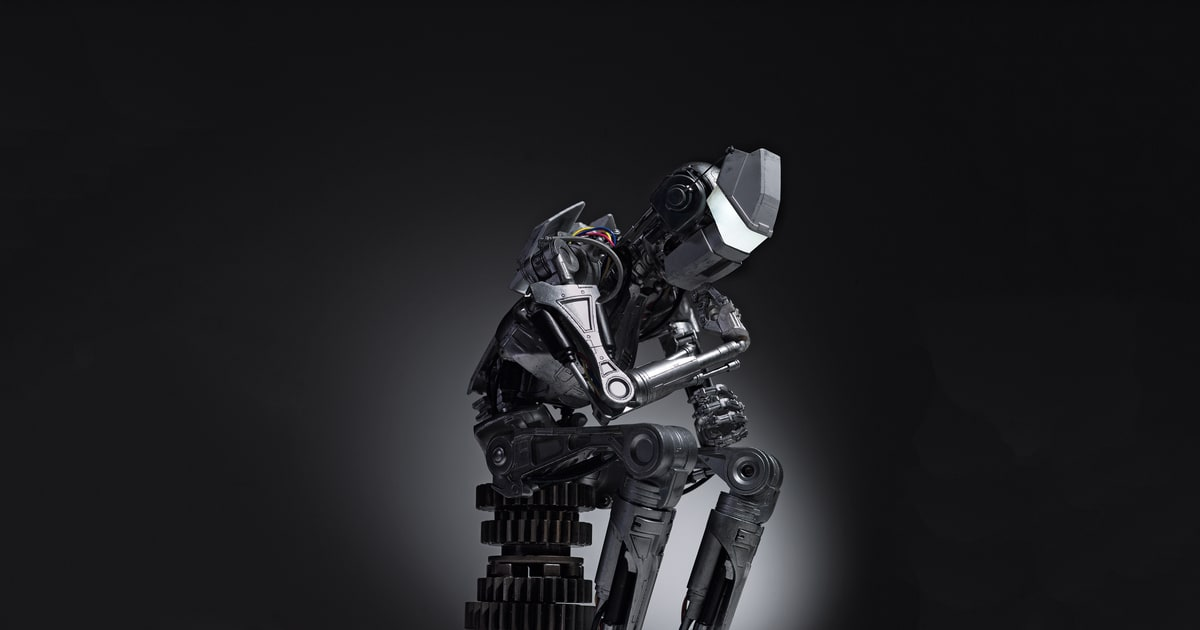
\includegraphics[width=0.75\paperwidth]{Scriptie/imgs/augmented-intelligence.jpeg}
                  
%                    %% Print the author at the bottom 
%                   \vspace{0.2\paperheight}
                  
%                  {\color{white} \fontsize{24}{48}\selectfont \textbf{\theAuthor} }
%             \end{center}
%         \end{minipage} 
%     \end{center}
   
%     \restoregeometry    
% \newpage

\maketitle

\begin{abstract}
    \noindent Training neural networks for robotics with real-world data can be a timely and potentially expensive task. However, many real-world environments can also be simulated inside of modern 3D rendering engines, with Unity being a great and versatile example. 
    With the use of these virtual simulations, artificial intelligence applications can be trained with a greater number of simulated edge-cases together with a reduction in costs. 
    This paper demonstrates the potential of using virtual environments by training a model that can determine the position of a robot on a football field. Furthermore, the virtual environment can simulate many different lighting conditions, which are difficult to capture in a dataset that only contains real-world data. This virtually generated dataset will then be used to train a neural network that can determine the robots position on the football field. The concept and benefits of generating a bird's eye view model in order to predict a location on the football field will also be explored. However, the bird's eye view model was not successfully implemented.\\
    Using virtual environments to train neural networks to be used with robotics is not a new concept. Frolov et al.\cite{1} proposes a pipeline that can generate virtual images in order to train convolutional neural networks.\\
    This thesis proves that using virtually generated datasets can improve the accuracy of models, specifically models that classify uncommon objects that are difficult to capture in large quantities in real-world datasets.\\
    The results of this thesis show that a machine learning model can be fitted on artificially generated data in order to predict a location on a football field with a two time improvement over making random guesses. However, for it to be used in practice, improvements still have to be made.
    
    % TODO: WRITE ABOUT RESULTS
    % https://augmentedtrader.wordpress.com/2012/02/07/8-elements-of-successful-abstracts/

\end{abstract}

\tableofcontents

\chapter{Introduction}
    The Dutch Nao Team\footnote{\url{https://www.dutchnaoteam.nl/}} is a team of students from the University of Amsterdam that competes in the Standard Platform League (SPL) of the RoboCup. The RoboCup\footnote{\url{https://www.robocup.org/}} is an annual football tournament where teams from all over the world come to compete. The RoboCup competition was created in order to stimulate research in robotics, with the end goal of beating a team of human football players with a team of robotic football players by the year 2050. The teams in the SPL all compete with the same humanoid robots, namely the NAO V6 robots made by Aldebaran\footnote{\url{https://www.aldebaran.com/en/nao}}. Figure 1.1 shows an example of the robots from two teams in the SPL playing football. The fact that every team has access to the exact same hardware means that the SPL is exclusively a software programming competition, which makes it a suitable platform for developing artificial intelligence solutions to problems such as localisation or team play.
    \hfill \break \\
    There are many challenges to overcome in order to program a robot that can play football \cite{challenges}, such as detecting the ball or determining the robot's location on the field. In the current state of the art, these aforementioned problems are solved with machine learning algorithms. In order for these machine learning algorithms to perform well, they require a lot of training data \cite{KornblithShlensLe2019}. This data is often gathered as real-world data, such as images of real robots or data saved from test matches. The problem with these real-world datasets is that they often lack the desired variance. If a large proportion of the data in the real-world dataset has been recorded in the same building for example, then the background and lighting conditions will likely be similar across the entire dataset. This is not desired when programming a robot that can perform well in competitions, as most venues offer different conditions that could not be included in the training data.
    \hfill \break \\
    Virtual environments offer a great potential solution to increase the performance of a machine learning algorithm. \cite{virt} for example proposes a method of navigating real-world spaces by training a machine learning model that uses data gathered from Google Earth. The potential benefits of using a virtual environment to generate a dataset are the cost effectiveness, the ease of generating a high quantity of data in a short amount of time and the potential increase in variance of the data. In a virtual environment it is also possible to include edge-cases that would normally be a rare occurrence in real world scenarios. Therefore a virtually generated dataset could enhance the performance of a machine learning algorithm on handling edge-cases that are rarely occur in real-world datasets \cite{edge}.   
    \hfill \break \\
    This paper will focus on creating a machine learning algorithm that can locate a robot on the football field. The training data for this machine learning algorithm will be generated in a virtual environment, made in the Unity 3D engine, that mimics the Intelligent Robotics Lab at the University of Amsterdam. The Unity perspective plugin \cite{unity} will be used to generate a dataset with many different perspectives of randomly generated locations on the football field, as well as randomly generated lighting conditions. The goal of this paper is to show that virtual environments can be used to generate datasets, which in turn can be used to develop machine learning algorithms.
    \hfill \break \\
    \begin{figure}[H]
    \centering
    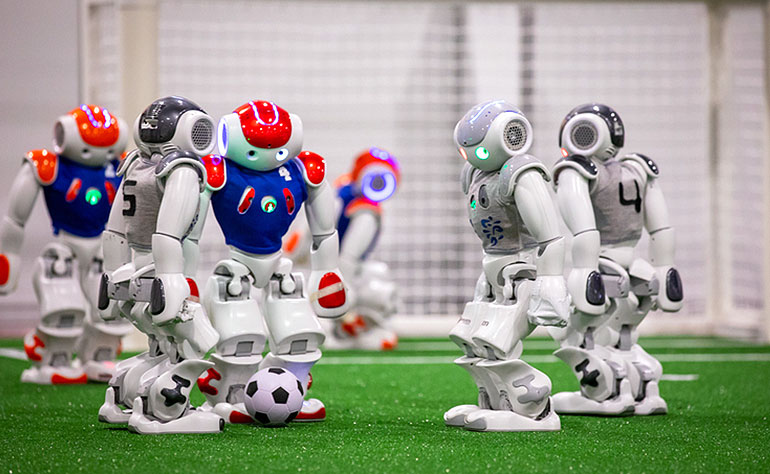
\includegraphics[width=0.95\textwidth]{Scriptie/imgs/robosoccer.jpg}
    \caption{Nao robots competing in the Standard Platform League at the 2022 RoboCup.}
    \end{figure}
    % \todo{implement research questions?}

\chapter{Theoretical background}
    In order to understand the context of this thesis, a theoretical background must first be framed. First, a state-of-the-art on the current use of virtual environments to generate datasets that are then used to train machine learning models will be sketched, followed by an explanation of the virtual environment used in this thesis. Secondly, the current localisation method of the Dutch Nao Team will be explored, including the weaknesses of the implementation and the reasons for this thesis to propose improvements to the localisation implementation. Finally, the process of generating a bird's-eye view image and training a machine learning model to predict the location on the football field will be explored. 
    
    \section{Virtual environments}
        Cao et al.\cite{6impose} proposes a method for improving the accuracy of robotic grasping of objects by addressing the "reality gap" between training in simulation and using the model in the real world. The paper focuses on the problem of estimating the 6D pose (position and orientation) of objects in cluttered scenes. Changes in lighting conditions and the clutter of the objects make this a difficult task that requires a lot of varied training data in order for the model to perform well.\\
        The proposed method, called 6IMPOSE, involves training a deep neural network to estimate the 6D pose of objects from artificially generated data in a virtual environment. The network is then fine-tuned on real-world data so that the model can still perform well when there are differences between the artificial data and the real world scenario. The resulting model outperforms other models that it was compared to in terms of accuracy and robustness to variations in lighting conditions.
        \hfill \break \\
        Peng et al.\cite{sim2real} proposes a method to improve the usability of simulated robotic controls in real-world applications. The paper addresses the reality gap by introducing dynamic randomisation during the simulation. This encourages the model to learn more robust and adaptable control strategies. The authors demonstrate the effectiveness of their approach on an object pushing task with a robotic arm. 
        This method presents a solution for improving the usability of machine learning models trained on virtual environments in the real world. It has the potential to overcome the limitations of existing simulation to real-world transfer methods and make it possible to train models on large amounts of simulated data with improved real-world performance.
        \hfill \break \\
        The Dutch Nao Team has previously experimented with generating artificial data in order to improve the ability to train machine learning networks. Lekanne gezegd Deprez \cite{hidde} proposes a method of using a GAN (Generative Adversarial Network) in order to generate realistic images that represent a real-world competitive scenario in the virtual SimRobot simulator \footnote{\url{https://github.com/HULKs/hulk}}. The SimRobot simulator provides a realistic environment that can be used to program new features for the robots. Lekanne gezegd Deprez \cite{hidde} also suggests that the use of virtual environments can reduce the amount of time it takes to annotate a dataset, as the ground truth can immediately be derived from the simulator environment. 

        % \todo{maybe also write about this paper's possible new findings in the field of simulations in order to generate datasets. Or how this paper approaches the reality gap problem.}

    \section{Virtual environment of the Intelligent Robotics Laboratory}
        The virtual environment that will be used in this thesis is a 3D Unity scene of the Intelligent Robotics Laboratory\footnote{\url{https://www.intelligentroboticslab.nl/}} at the University of Amsterdam, made by Joey van der Kaaij. Figure 2.1 provides an overview of the virtual environment. Within this environment, virtual robots and virtual cameras can be placed. Figure 2.2 depicts the view from a virtual robot at the center spot. The camera's parameters have been manually set to represent the top camera from a NAO V6 robot\footnote{\url{http://doc.aldebaran.com/2-1/family/robots/video\_robot.html}}.
        % The intrinsic camera matrix of this virtual robot's camera has been made to represent the top camera of a NAO V6 robot\footnote{http://doc.aldebaran.com/2-1/family/robots/video\_robot.html}.
        
        \begin{figure}[!tbp]
          \centering
          \begin{minipage}[b]{0.45\textwidth}
            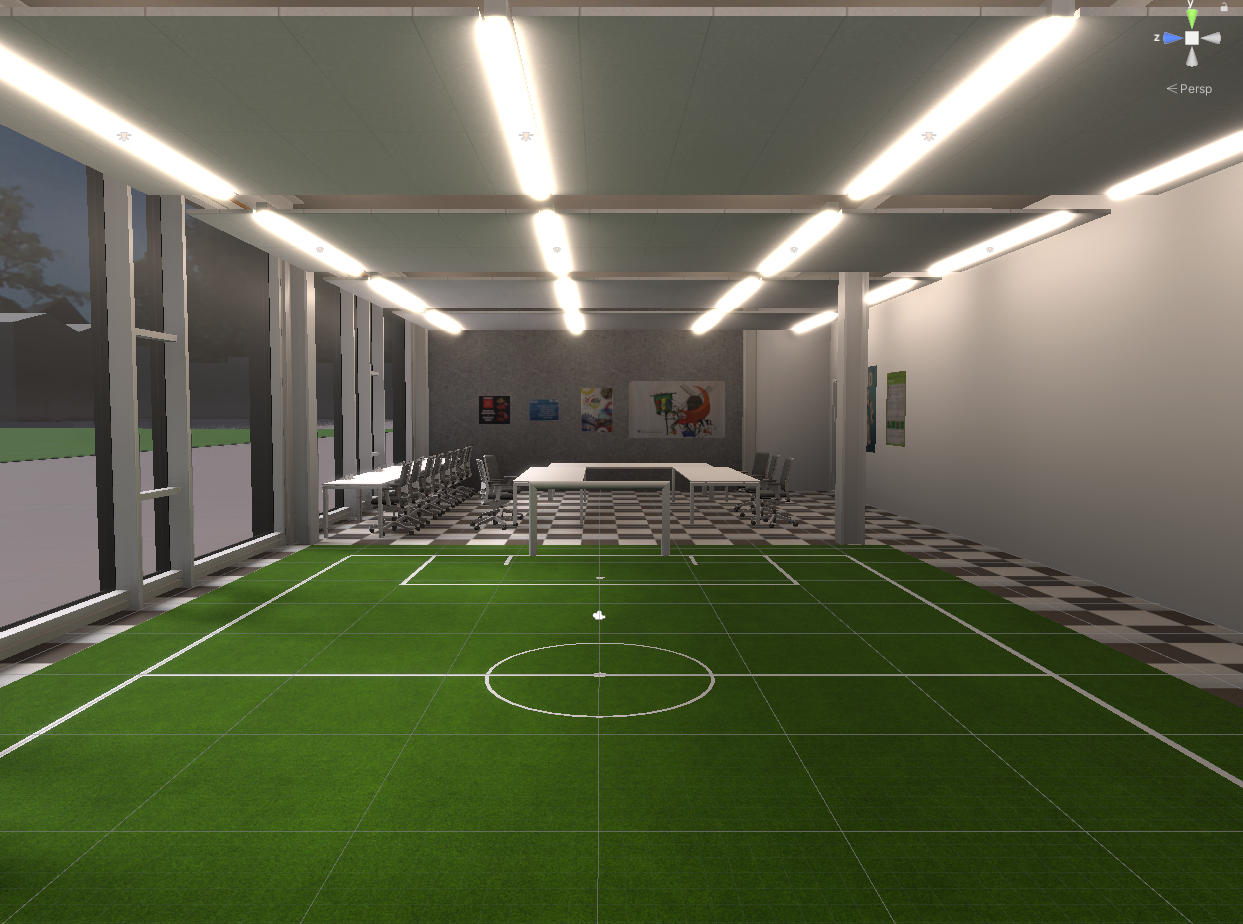
\includegraphics[width=\textwidth,height=50mm]{Scriptie/imgs/environment.png}
            \caption{Virtual environment of the Intelligent Robotics Labaratory at the University of Amsterdam.}
          \end{minipage}
          \hfill
          \begin{minipage}[b]{0.45\textwidth}
            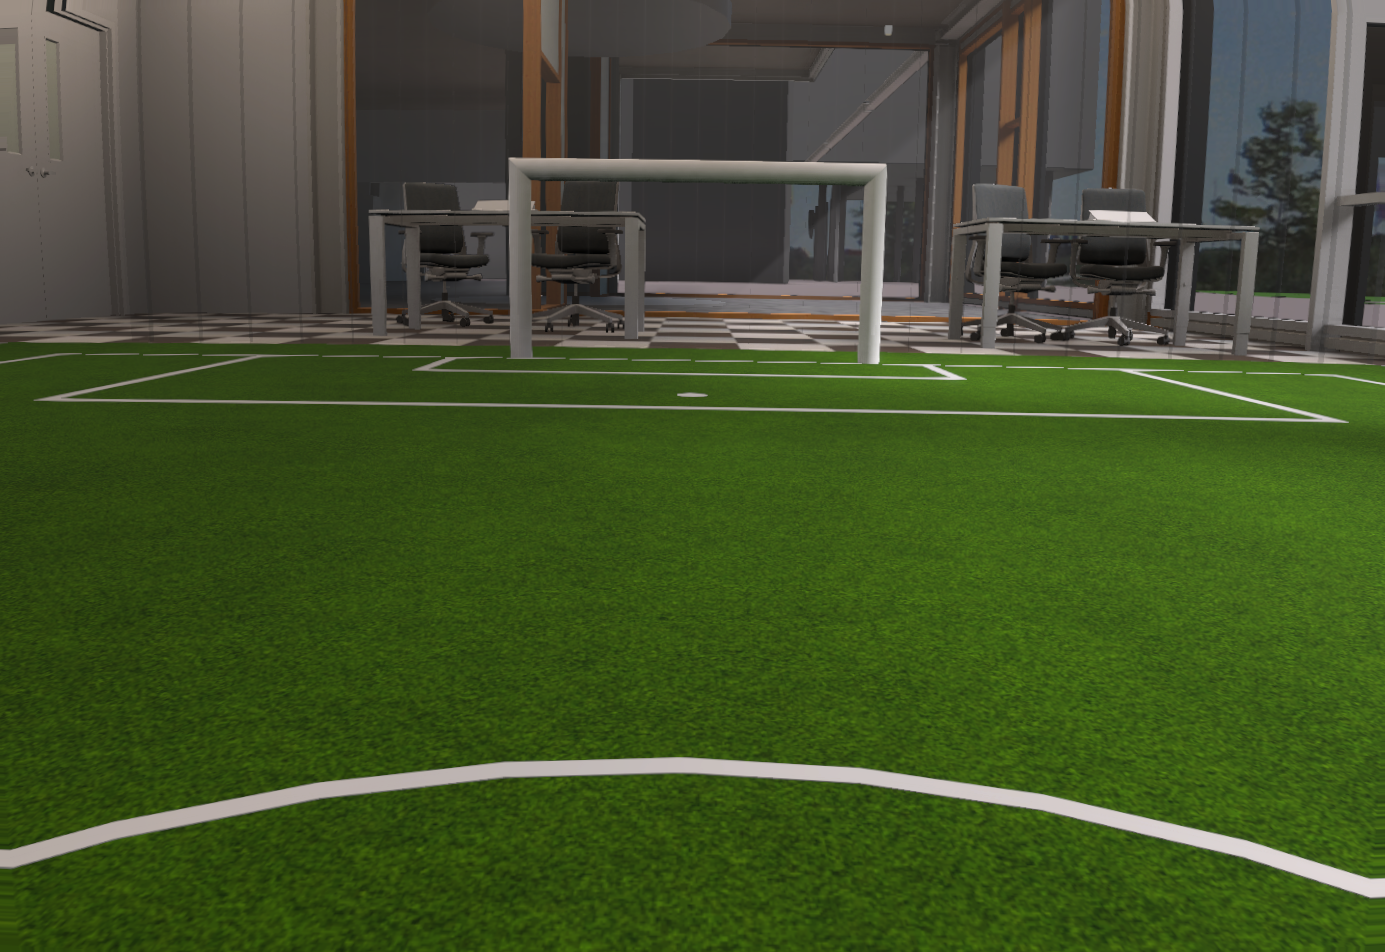
\includegraphics[width=\textwidth,height=50mm]{Scriptie/imgs/robot_cam.png}
            \caption{View of the virtual robot's camera.}
          \end{minipage}
        \end{figure}

        \subsection{Coordinate system of the virtual football field}
            \begin{figure}[H]
            \centering
            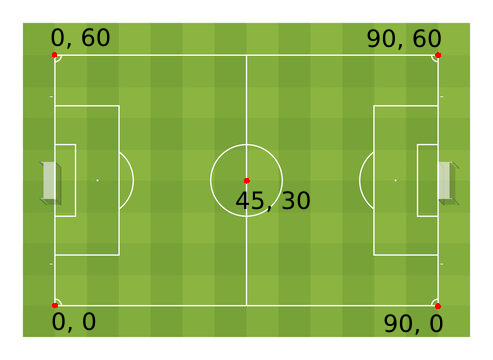
\includegraphics[width=0.67\textwidth]{Scriptie/imgs/360_F_378739470_y5Q7Z7ztxKDGPvnbf6l6gmP7JOMl4Dwt.png}
            \caption{(x, y) coordinate system of the football field, as defined by the coordinates of the four corners and the centre dot.}
            \end{figure}
            In order to predict a position on the football field with a machine learning model, the coordinate system must first be defined.
            The default origin, (0, 0), is the centre dot of the football field. This is not optimal, as it allows for both positive and negative values along the $x$ and $y$ axes. Shifting the origin to the bottom-left point of the football field ensures that only positive values are used for the position coordinates. This allows for an easier debugging process, as negative values instantly indicate an error. The resulting coordinate space is depicted in Figure 2.3.
            The real-world equivalent unit of these coordinates is decimetres. The football field in the Intelligent Robotics Laboratory, which the football field of the virtual environment is modelled after, is 9 by 6 meters in size.
    
        \subsection{Unity Perspective plugin}
            The virtual environment makes use of the Unity Perspective plugin, as proposed in \cite{unity}. This plugin allows parameters in the virtual environment to be changed with uniform random values. This allows for the camera to traverse the football field and take a picture at many randomly chosen locations. Furthermore, it allows for the lighting conditions to be changed randomly. Both the natural light, created by the sun and possibly diffused by the clouds, as well as artificial light, created by ceiling lamps, can be randomly changed. The plugin also makes use of deterministic randomness, which allows multiple runs to be similarly generated, but for example with a different amount of robots on the field.

     \section{Current localisation method of the Dutch Nao Team}
        The Dutch Nao Team currently uses a method of localisation that relies on detecting lines of the football field in the image captured by the robot's cameras, as described in \cite{DNT2018} and \cite{dnt2020}. However, this method is very susceptible to changes in lighting conditions, camera shake caused by the movement of the robot and the distance to the lines in the field.
        The reason for these inaccuracies are the localisation algorithm's dependencies on properly detecting white pixels in the images captured by the robot's cameras. However, the intensity of these pixels can change depending on the exposure of a given frame. If a frame is underexposed, some pixels of a line may be cut off by the line detection algorithm for not having a high enough exposure. If the pixels are overexposed, green pixels from the field may blur over into the white pixels from the lines or vice-versa. It is also possible for some false-positive segments to occur when the lighting conditions are unfavourable. Chromatic aberration and incorrect exposure could result in pixels that are not part of a line to be picked up by the segmenting algorithm.
        Motion blur introduced by the walking of the robot or the turning of the robot's head also negatively impact the image captured by the robot's cameras. One part of a room might be properly lit, but when the robot turns, its perspective could change to be too dark or too bright. The Dutch Nao Team has experimented with an automatic camera exposure algorithm \cite{dnt2022}, but this currently only sets the exposure values at the start of a match, which does not solve the changes in exposure during movement. Furthermore, this implementation is specifically designed to expose objects so that the object detector can detect them properly. It does not place a high weight on parts of the image that contain lines. 
        \hfill \break \\
        In order to improve the localisation of the robot, a machine learning approach can be taken. A machine learning implementation could have the following benefits:
        \begin{itemize}
            \item \textbf{Flexibility} Machine learning algorithms can be trained to be more flexible than a localisation method that relies on detecting lines. A machine learning model can be trained with many different lighting conditions, which can reduce the reliance on properly exposed environments \cite{flex}.
            \item \textbf{Robustness} A machine learning model can handle noisy or incomplete data better than a line detection method, and can therefore be more robust \cite{robust}. For example, a robot may lose sight of the field lines due to obstacles or other robots, but a machine learning algorithm can still predict its position based on other contextual cues such as the positions of other players.
            \item \textbf{Accuracy} Machine learning algorithms can be trained on large datasets to achieve high accuracy in predicting a robot's position \cite{accuracy}. In contrast, a line detection method may be susceptible to errors caused by variations in line thickness or colour, which can affect its ability to accurately determine the robot's position.
        \end{itemize}

    
     \section{Generating a Bird's-Eye-View}
        A bird's-eye-view perspective is a viewpoint that looks down onto a subject from above, as if seen from the height of a flying bird. This perspective can provide an increase in situational awareness \cite{sitaware}.
        % This paper will use the generated bird's-eye-view perspective to train a machine learning algorithm to predict the robot's location on the field. why?
        Furthermore, a bird's-eye-view perspective can generate a height map of the environment \cite{liftsplatshoot}. This height map can be used as a cost map in path-finding algorithms. A peak in the height-map might indicate a robot, and a hill might indicate the ball. The Dutch Nao Team currently implements a path-finding algorithm that generates a cost map based on detected objects in the robot's cameras \cite{rogier}. A bird's-eye-view perspective could enhance the cost-map, and therefore potentially increase the robot's ability to correctly choose a path across the field.   
        \hfill \break \\
        % \section{Lift-Splat-Shoot}
        The Lift-Splat-Shoot algorithm proposed in \cite{liftsplatshoot} provides a method of generating a bird's-eye view perspective from an arbitrary number of cameras.
        The method involves three main steps: lift, splat, and shoot. In the lift step, the image's pixels are lifted, or transformed, into a 3D representation. In the splat step, the lifted 3D points are projected onto a regular 3D grid using a differentiable, weighted summing operation. Finally, in the shoot step, the 3D grid is fed through a neural network to produce an encoded representation of the image.
        
        Philion and Fidler \cite{liftsplatshoot} proposes a method of generating bird's-eye-view perspectives for arbitrary camera rigs. However, this thesis will only use a single camera, namely the view from the top camera of the Nao V6 robot. This means that this thesis will focus on the scenario where $n$ RGB images are given: ${X_k \in \mathbb{R}^{3 x H x W}}$ Each image has an intrinsic camera matrix $I_k \in \mathbb{R}^{3 x 3}$ and an extrinsic camera matrix $E_k \in \mathbb{R}^{3 x 4}$. Since this thesis only uses a single camera, the rasterized representation of the scene in the bird's-eye-view coordinate frame will have the form of: $y \in \mathbb{R}^{3 x X x Y}$, as there are 3 colour channels in the $n$ RGB images.
        The following sections will provide a more in-depth explanation into the workings of the lift-splat-shoot algorithm.

        \subsection{Lift}
            \begin{figure}[H]
            \centering
            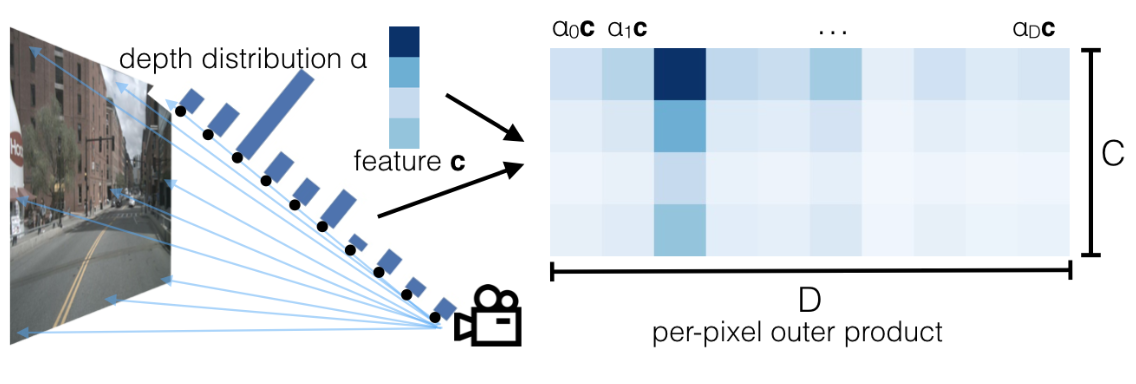
\includegraphics[width=0.85\textwidth]{Scriptie/imgs/Screenshot 2023-05-16 at 13.25.30.png}
            \caption{Visualisation of the "lift" step. For each pixel, it predicts a distribution over depth $\alpha \in \Delta^{D-1}$ (left in Figure 2.4) and a context vector $\textbf{c} \in \mathbb{R}^C$ (top-left in Figure 2.4). Features at each point along the ray are determined by the outer product $\alpha$ and \textbf{c} (right in Figure 2.4) \cite{liftsplatshoot}}
            \end{figure}

            The goal of the lift part is to \textit{lift} each image from a local 2-dimensional coordinate system into a 3-dimensional frame that is shared across an arbitrary number of cameras. 
            When using multiple cameras, depth is required to fuse the images together. However, it is not possible to know the "depth" of a pixel as an a-priori value. Therefore, the authors of the lift-splat-shoot paper propose a method of generating representations at every possible depth for every pixel in the image.
            This is done with the following method: Let $X \in \mathbb{R}^{3 x H x W}$ be an image, and let $p$ be a pixel in the image with the image coordinates $(h, w)$. Now it is possible to choose $|D|$ points ${(h, w, d) \in \mathbb{R}^3 | d \in D}$ at each pixel where $D$ is a set of discrete depths. This results in a point cloud with a size of $D$ x $W$ x $H$.
            This point cloud can then be given to a network in order for the network to predict the depth of the image. At pixel $p$, the network predicts a context $c \in \mathbb{R}^C$ and a distribution over depth $\alpha \in \Delta^{|D|-1}$ for every pixel. A given feature $c_d \in \mathbb{R}^C$ at point $p_d$ is then defined as the context vector for pixel $p$ scaled by $\alpha_d$, resulting in $c_d = \alpha_dc$. A visual example can be found in Figure 2.4.
            % \todo{I only plan on using a single camera. Will the lift-splat-shoot algorithm even be possible? If it requires multiple point clouds from multiple different cameras to merge into a single 3D coordinate system, then a single camera will not be enough.}
        
        \subsection{Splat}
            \begin{figure}[H]
            \centering
            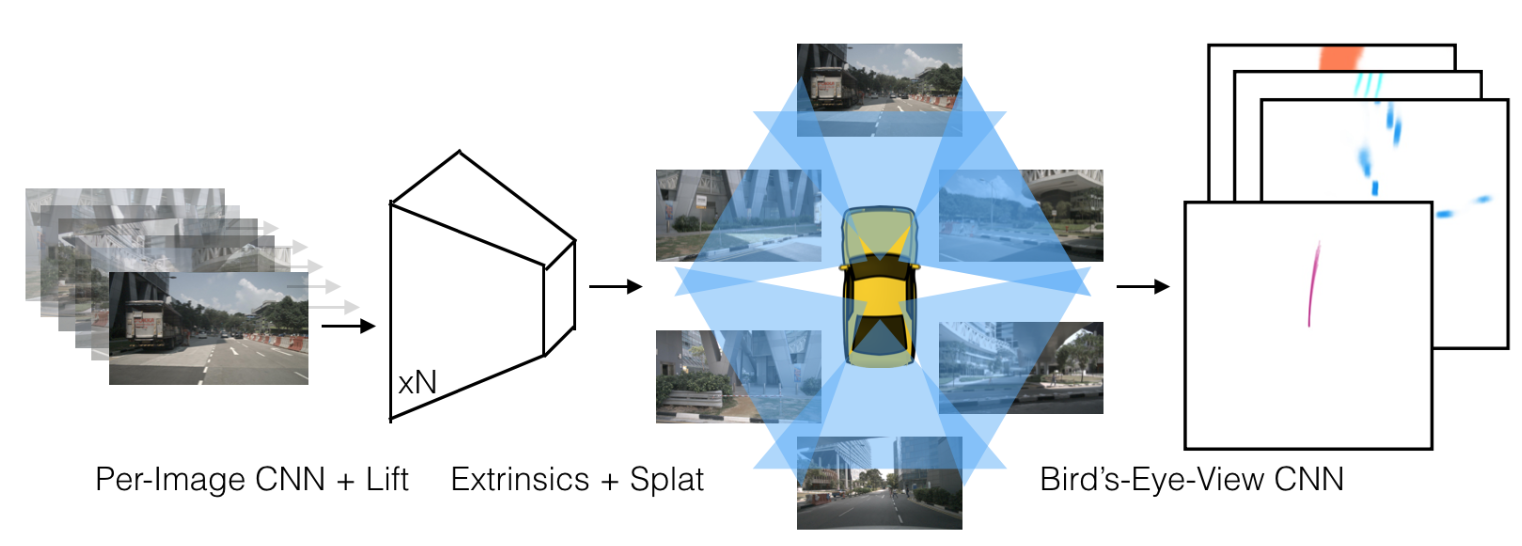
\includegraphics[width=0.85\textwidth]{Scriptie/imgs/Screenshot 2023-05-16 at 16.03.41.png}
            \caption{The lift-splat-shoot algorithm takes as input $n$ images (left in figure 2.5) and their
                corresponding extrinsic and intrinsic parameters. In the “lift” step, a frustum-shaped
                point cloud is generated for each individual image (center-left in Figure 2.5). The extrinsics and
                intrinsics are then used to splat each frustum onto the bird’s-eye-view plane (center-
                right in figure 2.5). Finally, a bird’s-eye-view CNN processes the bird’s-eye-view representation for
                BEV semantic segmentation or planning (right in Figure 2.5). \cite{liftsplatshoot}}
            \end{figure}

            The goal of the Splat part of the lift-splat-shoot algorithm is to project each frustum-shaped point cloud, which are generated for every image, onto the bird's-eye-view plane. 
            The lift-splat-shoot algorithm uses the pointpillars architecture, as proposed in \cite{pointpillar}. This architecture can convert the point cloud output of the lift step into "pillars". These pillars are voxels with infinite height. Every point cloud gets assigned to the nearest pillar and sum-pooling is performed to create a C x H x W tensor. Philion and Fidler \cite{liftsplatshoot} proposes a more efficient method of performing the sum-pooling operation, called the "Frustum Pooling Layer". This improved method lowers memory usage and increases the speed of the sum-pooling operation. The resulting tensor can then be processed by a CNN. The Splat process is visualised in Figure 2.5.

        \subsection{Shoot}
            The goal of the Shoot part of the lift-splat-shoot algorithm is to generate a diverse set of samples representing potential solutions. This phase aims to explore the solution space and capture a wide range of possible solutions. By generating a diverse set of particles, the shoot phase enables the lift-splat-shoot algorithm to search for optimal or near-optimal solutions. The goal is to avoid getting trapped in local optima, but instead promote thorough exploration of the solution space. By generating a variety of samples, the lift-splat-shoot algorithm increases its chances of finding better solutions and improves the overall effectiveness of the optimisation process. Additionally, the shoot phase enables the lift-splat-shoot algorithm to sample different regions of the solution space, ensuring that a wide range of potential solutions is considered.
            % \todo{incorporate the maths}
        % \subsection{Data augmentation}
            % post\_rot and post\_trans matrices

        % \section{other methods}

        % \section{Reliance on the nuScenes dataset}
        
     \section{Using a neural network to predict a position}
        Predicting the position of a robot on the football field using a machine learning model that has been trained on artificial data is the main goal of this thesis. Therefore, the theory behind predicting a location using a machine learning algorithm must first be explored.
        \hfill \break \\
        Pedrazzini \cite{posest} proposes a method of estimating the positions of 3D objects on a football field. It focuses on finding the 3D coordinates of a ball on a 2D image of the football field. The authors propose using a Convolutional Neural Network (CNN), instead of using the geometrical computer vision solution \cite{ex1} \cite{ex2}. This traditional solutions almost always follow the same general steps: \begin{enumerate}
            \item Computing the projection matrix.
            \item Detecting the object within the image.
            \item Estimating the 3D position of the object.
        \end{enumerate}
        Pedrazzini \cite{posest} instead proposes a method that relies on machine learning. It lists the following steps to train and evaluate a machine learning model that can predict the 3D coordinates of a ball: \begin{enumerate}
            \item \textbf{Collecting data:} creating a comprehensive dataset to train and test the designed models.
            \item \textbf{Define a model to solve the task:} iterating over the assumptions and configurations a deep learning model should be designed to predict the labels accurately.
            \item \textbf{Tune the parameters:} adjusting the hyper-parameters for better performances.
            \item \textbf{Analysing the results:} reflecting over the obtained scores to possible further improvements.
        \end{enumerate} 
        These steps are very broadly applicable too most machine learning implementations. The authors have intentionally made these steps very broadly applicable in order to create a flexible and scalable method. 

        \subsection{Using a Convolutional Neural Network}
            \begin{figure}[H]
            \centering
            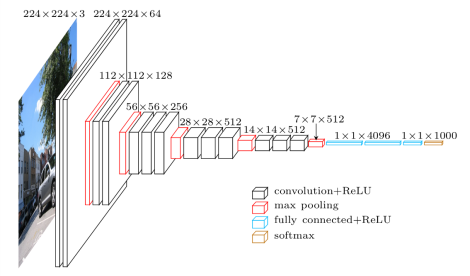
\includegraphics[width=0.9\textwidth]{Scriptie/imgs/vgg_7mT4DML.png}
            \caption{Visual representation of the CNN used in the VGG architecture. Different coloured layers represent the different types of layers commonly found in a CNN. The colour that represents a specific layer can be found in the legend in the bottom right corner of the image. \cite{Explained}}
            \end{figure}
            A convolutional neural network (CNN) is a type of machine learning algorithm designed to process and analyse data with a grid-like structure, such as images. It is commonly used in computer vision tasks, such as: image classification, object detection, and image segmentation \cite{cnn}.\\
            The main building blocks of a CNN are convolutional layers, pooling layers, activation functions and fully connected layers. A CNN starts with an input layer. This layer takes in an image as input. Next are the convolutional layers. These layers perform convolution operations on their input by taking the convolution of the input with a kernel, these convolution kernels are also often referred to as filters. Within the convolutional layer, the filters slide across the input, multiplying the filter weights with the corresponding input values. This results in a feature map that highlights important spatial patterns in the input. Activation Functions, typically a non-linear activation function like a Rectified Linear Unit (ReLU) \cite{relu} is applied to the feature maps. This introduces non-linearity and allows the CNN to learn complex relationships. Pooling layers are often used in between convolutional layers. These layers reduce the spatial dimensions (width and height) of the feature maps while conserving important information. Pooling techniques that are often used include max pooling, which takes the maximum value within each pooling region, and average pooling, which calculates the average of a pooling region. After the input has progressed through the convolutional and pooling layers of the CNN, it reaches a fully connected neural network. This layer flattens the feature map and passes it through one or more fully connected layers. These layers are similar to those in traditional neural networks and are responsible for learning higher-level representations and making predictions. After the input has gone through all the layers of the CNN, it reaches the output layer. This output layer is used to determine the 'result' of a pass through the CNN. Figure 2.6 gives a visual representation of how a CNN can be constructed of the different kind of layers. The CNN depicted in Figure 2.6 is the Very Deep Convolutional Networks for Large-Scale Image Recognition (VGG), as proposed in \cite{vgg}.

        % \subsection{GoogLeNet}

\chapter{Method}
    This chapter will detail the steps that were taken in order to predict a robot's position on a football field. It will begin with explaining the steps that are required to generate the dataset, as well as proving the variance of the dataset. Secondly, it will discuss the steps that were taken to generate a bird's eye view perspective, as well as highlighting the problems that arose while implementing the bird's eye view perspective and how those problems could be solved in future research. Finally, this chapter will explain the steps taken to train and validate a convolutional neural network in order to predict a location. 

    \section{Generating a dataset in Unity}
        \begin{figure}[H]
        \centering
        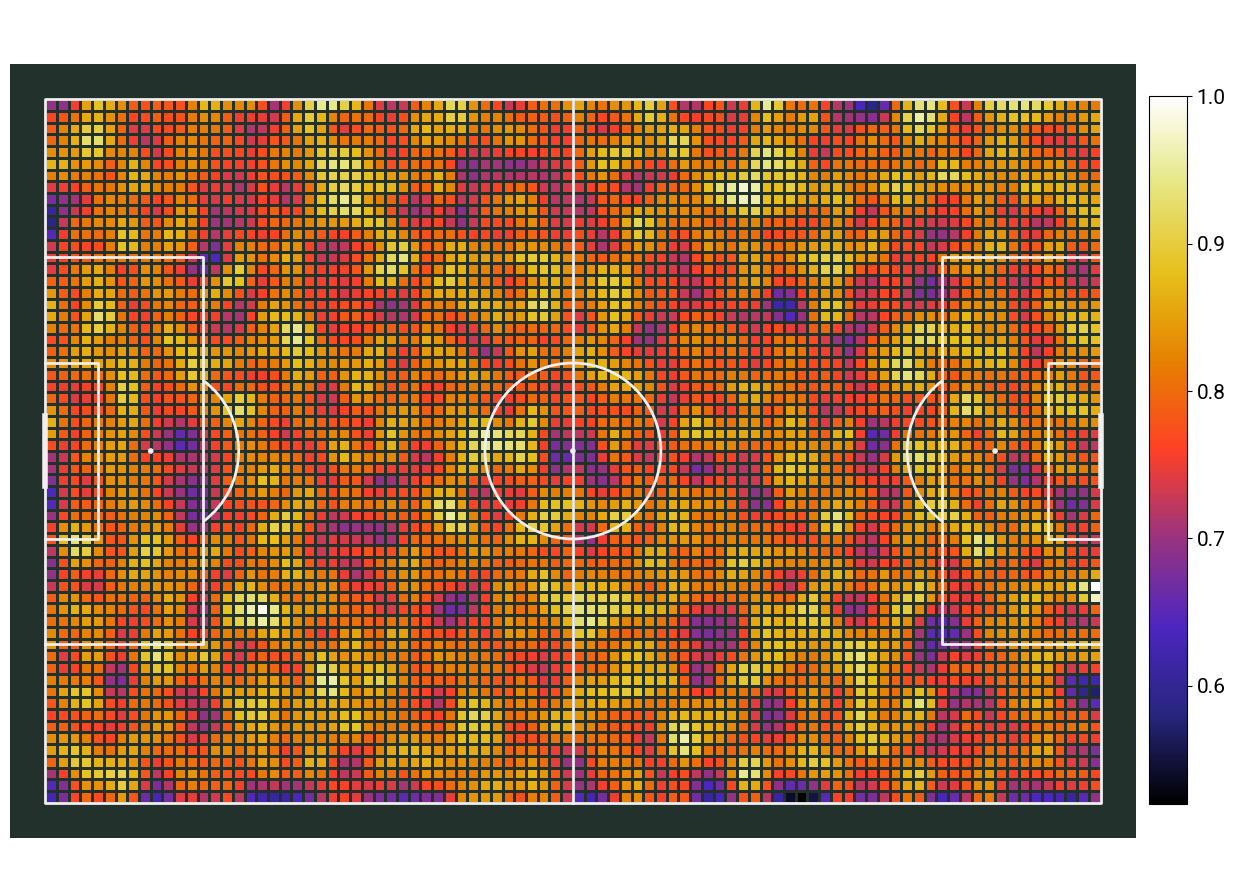
\includegraphics[width=0.95\textwidth]{Scriptie/imgs/100kpos2.png}
        \caption{Normalised distribution of randomly generated positions by the Unity Perspective plugin, N=100.000}
        \end{figure}
        
        The first step to generating a dataset in Unity is to set the parameters of the Perspective plugin to the correct values. First, the parameters of the Transform Randomiser Tag of the virtual robot's camera are set correctly. As displayed in Figure 2.2, the starting position of the camera is the centre dot of the football field. Therefore, the camera must be able to move 45 units in the positive and negative $x$ axis and 30 units on the positive and negative $y$ axis. 
        Figure 3.1 shows a heat map of the distribution of locations the camera took an image. This Figure contains 100.000 samples and shows that the Transformation parameters are set correctly in order to capture images uniformly across the entire field.
        In order to capture a diverse set of images at the same location, the camera must also be rotated at every new capture. This is done by setting the rotation parameter of the virtual camera's randomiser tag. By setting the $y$ axis rotation of the camera to a random value between 0 and 360, the camera can be rotated to capture multiple different views at a single position. By setting the $x$ and $z$ axis rotation to a random value between -2 and 2 degrees, the robot's shake during walking can be captured in the dataset. Figure 3.2 shows how every example image has a different rotation compared to the starting position of the camera as depicted in Figure 2.2.

        \begin{figure}[H]
        \centering
        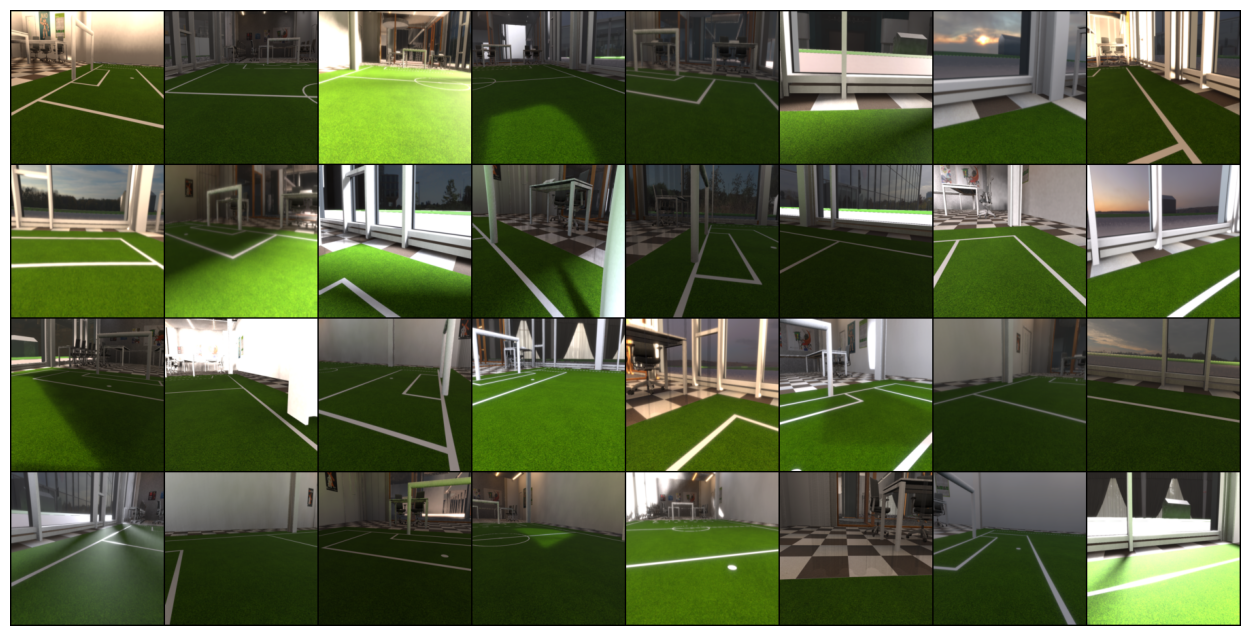
\includegraphics[width=0.9\textwidth]{Scriptie/imgs/previmage.png}
        \caption{32 example images generated by the Unity environment.}
        \end{figure}

        In order for the dataset to capture different lighting conditions, the \textit{SunAngleRandomiser}, \textit{SkyboxRandomiser} and \textit{LightRandomiser} tags can be used in the \textit{SCENARIO} object of the Unity environment. With these tags, the time of date, cloud coverage, sun intensity and angle can be randomised. These tags work together to randomly generate different lighting conditions for each sample. The results of these random lighting conditions are depicted in Figure 3.2. \\
        After the transformation, rotation and lighting parameters are set correctly, the amount of generated samples can be set with the \textit{iteration count} parameter of the \textit{SCENARIO} object.
        \hfill \break \\
        The Unity Perspective plugin generates datasets in the SOLO\footnote{\url{https://docs.unity3d.com/Packages/com.unity.perception@1.0/manual/Schema/SoloSchema.html\#:\~:text=A\%20SOLO\%20dataset\%20is\%20a,or\%20train\%20machine\%20learning\%20models.}} format. For every sample, it records the exact position, rotation and intrinsic camera matrix and saves these values to a JSON file, as well as a jpg image file that records the robot's view. The SOLO dataset format can easily be converted to a COCO\footnote{\url{https://cocodataset.org/\#home}} dataset format with the help of Pysolotools\footnote{\url{https://docs.unity3d.com/Packages/com.unity.perception@1.0/manual/Tutorial/convert_to_coco.html}}.
        
        % In order for this paper to show that artificial environments can be used to generate usable datasets, the validity of the dataset generated by the virtual environment must first be examined.

        % \begin{figure}[H]
        % \centering
        % 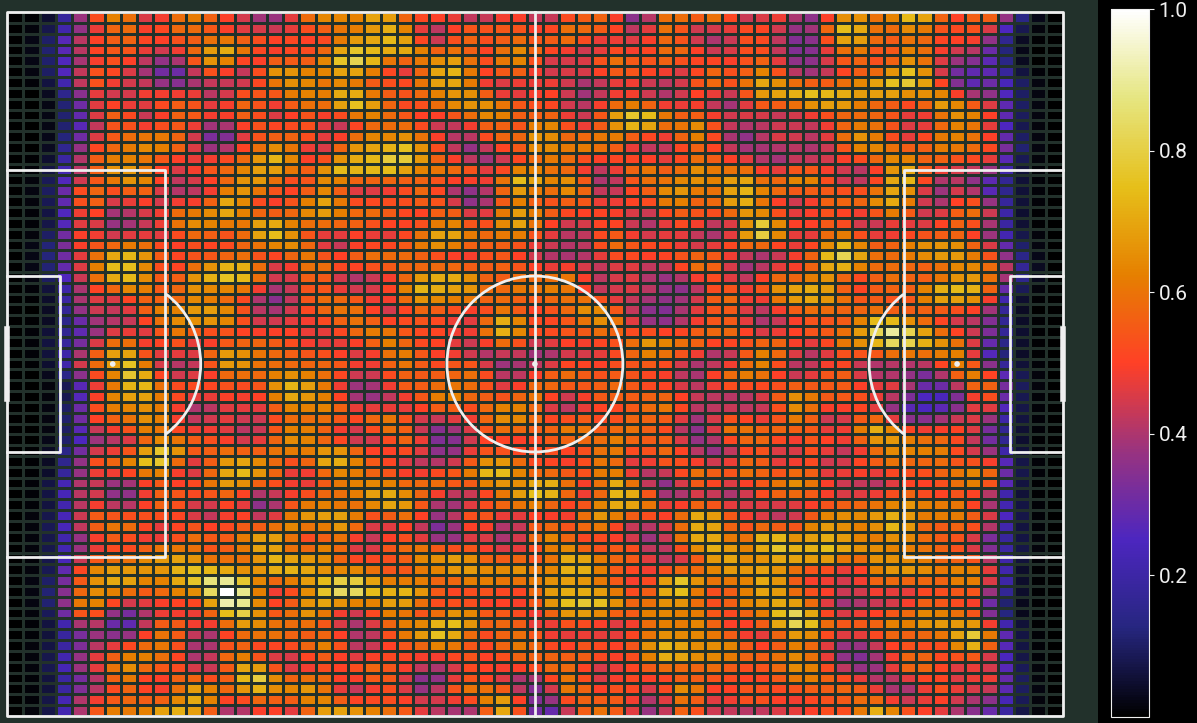
\includegraphics[width=1\textwidth]{Scriptie/imgs/10klightavg2.png}
        % \caption{Normalised distribution of lighting conditions generated by the Perspective plugin, N=10.000}
        % \end{figure}

    \section{Bird's-eye view perspective}
        This study has not successfully implemented a bird's-eye view model. However, the steps taken will still be discussed. 

        \subsection{Implementing Lift-Splat-Shoot}
            The implementation of the Lift-Splat-Shoot paper \cite{liftsplatshoot} can be found on this GitHub page\footnote{\url{https://github.com/nv-tlabs/lift-splat-shoot}}. This code was used in an attempt to generate bird's-eye view images with images captured by the virtual robot's camera. Using bird's eye view images instead of regular egocentric perspective images in order to determine a robot's position on the football field has the following advantages:
            \begin{itemize}
                \item \textbf{Decrease in training on environmental features:} When using images captured with an egocentric camera perspective, many environmental features will also be captured. This can be seen in Figure 3.2, where many example images also include part of the Intelligent Robotics Laboratory in the background. These environmental features can introduce points of interest for a machine learning model that are unique to a specific location. This might be beneficial when the location is known beforehand, but when a robot has to be localised on a football field at an arbitrary location, these environmental features are not beneficial to the accuracy of the predictions. A model trained on images with a bird's-eye view perspective can therefore perform better on images that are captured on football fields at arbitrary locations as the bird's-eye view model will create a representation where the environmental features can be ignored.
                \item \textbf{Increase in situational awareness:} The Lift-Splat-Shoot algorithm, as detailed in \cite{liftsplatshoot}, can produce segmented images directly from the bird's-eye view model. This allows for clear separation between field lines, other robots, the goal and irrelevant features such as background information. These segmented features can then also be used for object avoidance, as well as gathering extra information about the location of the ball and the robot's relation to the goals.
            \end{itemize}

        \subsection{Annotated dataset}
            The Lift-Splat-Shoot algorithm requires an annotated dataset in order for it to be able to segment different features of an image. Properly annotated datasets ensure that the algorithm can learn discriminative features and spatial relationships, enabling robust object recognition and segmentation. These annotations can be derived from the ground-truth of the Unity environment. The Unity Perspective plugin has the capability to generate bounding boxes around objects, and the Unity environment could be extended with the ability to clearly separate the field lines from the field itself, creating the possibility to clearly separate the lines from the field when annotating. These separated field lines could then be used as the main feature for the neural network to predict the robot's location on the field. 
            
        \subsection{Training Lift-Splat-Shoot}
            The Lift-Splat-Shoot algorithm trains on the following parameters: 
            \begin{itemize}
                \item \textbf{Image:} An arbitrary amount of RGB images.
                \item \textbf{Intrinsic camera matrix:} The intrinsic camera matrices of the cameras that took the RGB images.
                \item \textbf{Rotation:} The rotation matrices of the RGB image.
                \item \textbf{Transformation:} The transformation matrices of the RGB images.
                \item \textbf{Post\_rot:} Post rotation matrix, used in data augmentation. This parameter does not come from the dataset, but is randomly sampled.
                \item \textbf{Post\_trans:} Post translation matrix, used in data augmentation. This parameter does not come from the dataset, but is randomly sampled.
                \item \textbf{Binary image:} This parameter takes an image as input, extracts ego pose information, and processes the annotations in the image to generate a binary image where the region occupied by vehicles is marked with 1.0.
            \end{itemize}
            As stated in the listing above, The post\_rot and post\_trans matrices are used in data augmentation. If the use of data augmentation is not wanted, the post\_rot matrix can be set to an identity matrix and the post\_trans matrix can be set to a zero vector. Furthermore, every parameter can be a tensor of size N, where N is greater than 0. This is due to the fact that the Lift-Splat-Shoot algorithm proposes a method of using an arbitrary amount of cameras to generate a bird's-eye view. Therefore, each index of the tensor can hold information about one of the total number of cameras that were used to gather the data.

        \subsection{Reliance on the NuScenes dataset}
            Research in bird's-eye view models is often related to self-driving cars \cite{liftsplatshoot} \cite{ex1} \cite{ex2}. Self-driving cars rely on a combination of sensors such as LiDAR, cameras, and radar in order to perceive the surrounding environment. Bird's-eye view models provide a comprehensive representation that integrates information from multiple sensors, allowing for a holistic view of the surroundings. This is particularly useful in self-driving cars, where a detailed understanding of the environment is crucial for the car to be able to make a safe and reliable decision. However, the Nao V6 robot only has access to a top- and bottom view camera. This makes implementing a model that expects input from multiple different kinds of sensor difficult if there is no obvious method to focus solely on camera input. 
            \hfill \break \\
            The NuScenes dataset \cite{nuscenes} is an annotated dataset that provides comprehensive sensor data captured from a fleet of self-driving cars operating in various urban environments. The dataset includes a range of sensor types, such as: cameras, LiDAR, radar, and GPS data. This dataset is used as the benchmark to compare different bird's-eye view models\cite{liftsplatshoot}. Therefore, the implementation of these models are often programmed to interface exclusively with the NuScenes dataset, making it difficult process to adapt the proposed models in a different context. 

    \section{Training a model to determine a robot's position on the football field}    
        This section will detail the steps that were taken in order to train a machine learning model in order to predict a position of a robot on a football field. The model that will be discussed is GoogLeNet \cite{googlenet} \todo{I am currently also experimenting with Resnet 50, Resnet101 and EfficientNet in order to compare these different models and find out which model performs the best for this task}, which is a deep convolutional neural network with 22 layers.
        This section will first highlight the method of transforming locations of the football field into classes that GoogLeNet can identify, followed by an explanation of the training process. Furthermore, this section will conclude with an overview as to how a real-world verification dataset was recorded with the use of the Intelligent Robotics Laboratory's Optitrack\footnote{\url{https://optitrack.com/}} system. 
        \subsection{Dividing the football field into a grid}
            The first step is to divide the football field in a grid of individual squares, so that every square on the football field is a class for GoogLeNet to classify. This way, the determining of the position of the robot on the football field can be transformed into an image classification problem. 
            Equation 3.1 gives the formula as to how a $(x, y)$ coordinate is transformed to a single class. Note that the rounding operation is in theory not necessary, as the unity camera should never exceed the boundary of the football field in the virtual environment. However, in order to ensure there are no bugs when indexing the target vector of the model, the rounding operation is included. The constant of 91 is the width of the football field. Because the coordinates of 0 and 90 are both included as a possible location, the football field has a total width of 91.
            \begin{equation}
                f(x, y) = \lfloor{x + \frac{1}{2}} \rfloor + (91 * \lfloor y + \frac{1}{2} \rfloor)
            \end{equation}
            % Dividing the football field in grids gives the classification formula as listed in equation 3.2.
            % \begin{equation}
            %     \hat{a} = 
            % \end{equation}

        \subsection{Training GoogLeNet}
            GoogLeNet, as proposed in \cite{googlenet}, is a convolutional neural network that is based on the inception architecture, as also proposed in \cite{googlenet}. The inception architecture consists of multiple parallel convolutional layers, all with different sizes. The inception modules allow the network to capture features at multiple scales and abstract levels, allowing the model to learn more complex patterns and objects. Because the features of the location grids of the football field only differ sightly between classes, it is important that the model used is capable of picking up on abstract features. An entire overview of the architecture used can be found in Figure A.1.
            
            \begin{figure}[H]
            \centering
            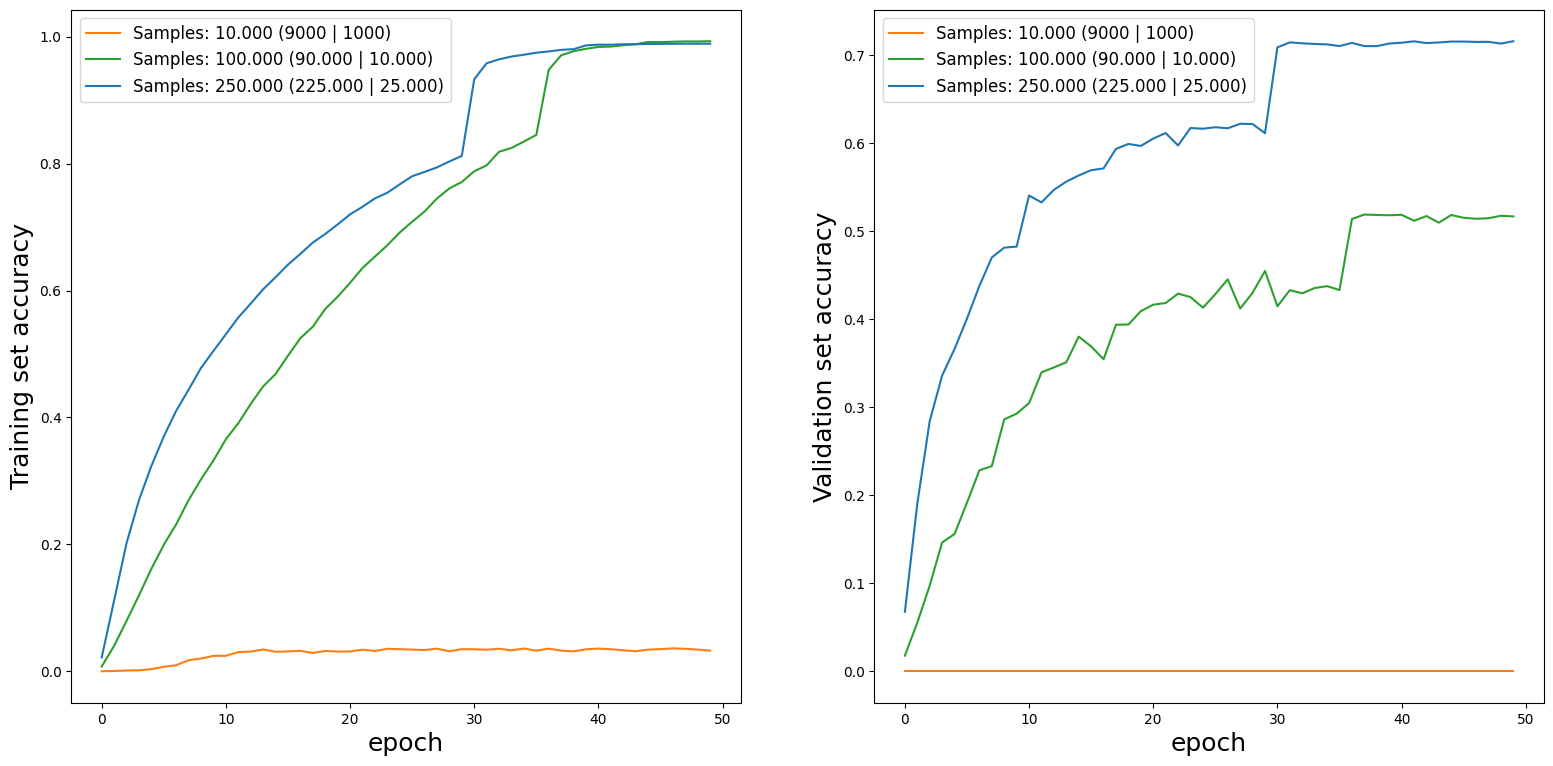
\includegraphics[width=1\textwidth]{Scriptie/imgs/testink.png}
            \caption{Training set and validation set accuracy of datasets containing a different number of samples. The split of the amount of samples that are in the training set and that are in the validation set are noted between the brackets.}
            \end{figure}
            
            \begin{figure}[H]
            \centering
            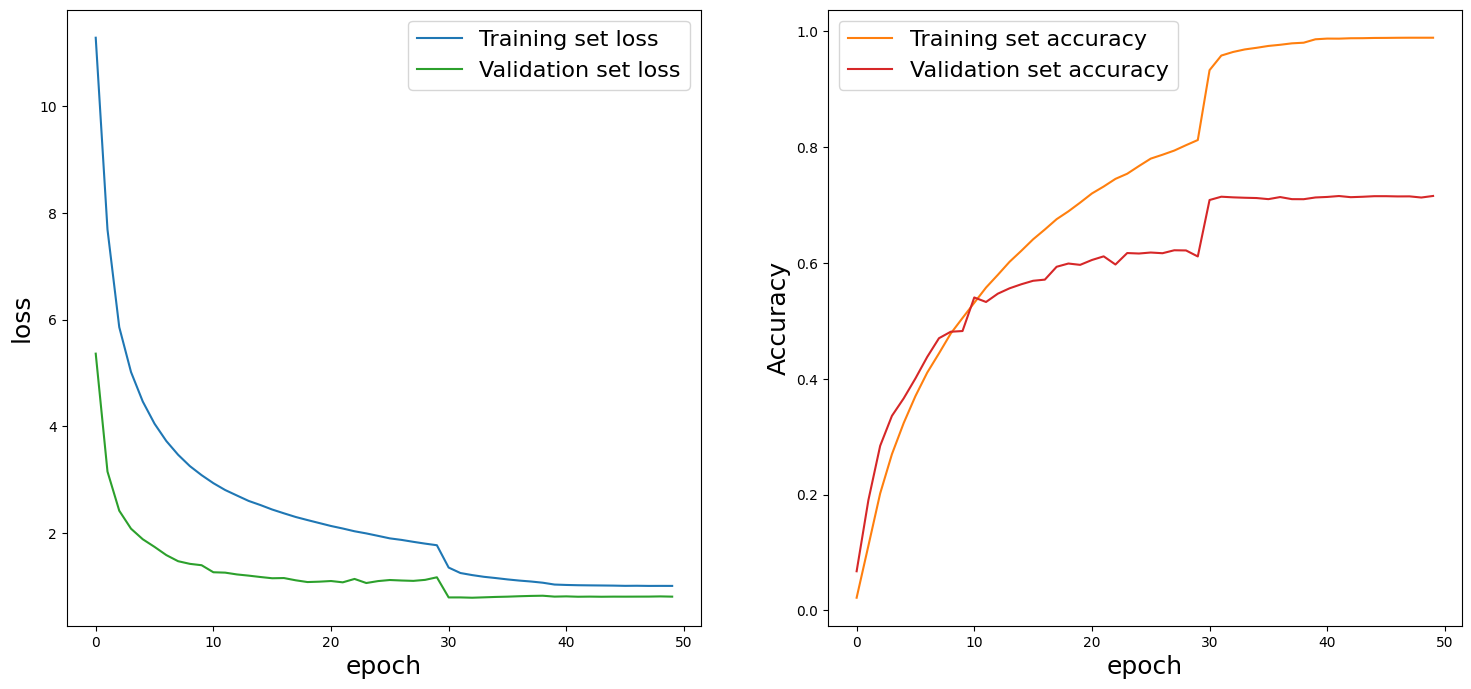
\includegraphics[width=1\textwidth]{Scriptie/imgs/isthisloss2.png}
            \caption{Loss and accuracy graphs of training GoogLeNet on 250.000 images with 50 epochs. The training set contained 225.000 samples and the validation set contained 25.000 samples.}
            \end{figure}

            In order for GoogLeNet to predict a robot's location on a football field, the model was trained on sample images generated by the Unity environment. Figure 3.3 shows the importance of the size of the dataset used. When a too small dataset is used, 10.000 samples for example, the model does not manage to find an appropriate fit. This is depicted in figure 3.3, where the orange line (10.000 samples) barely reaches above a 5\% fit. Furthermore, the validation set did not manage to achieve an accuracy above 0\% after training for 50 epochs. However, the model did manage to find an appropriate fit through the larger datasets. As shown in figure 3.3, a larger dataset will both produce a better fit, with a higher accuracy on the validation set as well as allowing the model to find a better fit faster. The dataset with 250.000 manages to maintain a better fit across every epoch over the dataset with 100.000 samples. Note that the jumps in accuracy around epoch 30 are because of the optimiser Adam\footnote{\url{https://pytorch.org/docs/stable/generated/torch.optim.Adam.html}} automatically changing the learning rate.
            Note that the model only counts a prediction as correct when it exactly matches the class of the input image. If the image is only one class off, which equates to 10 centimetres in the real world, the model will count the prediction as incorrect.
            \hfill \break \\
            Figure 3.4 plots the categorical cross-entropy loss of the model across epochs. Figure 3.4 does not show clear signs of overfitting. The curve of the training set accuracy does not make sudden, unexpected increases as the model trains for longer. However, a significant difference in accuracy between the training set and validation set appears around epoch 15. This could be a result of the dataset not being large enough. Figure 3.3 shows that the datasets of sizes 100.000 and 250.000 can both produce an almost perfect fit on the training set, reaching almost identical accuracies around epoch 40. However, their validation set accuracies differ significantly. 

        % \subsection{ViT}

        \subsection{Recording a real-world validation set with Optitrack}
            \begin{figure}[H]
            \centering
            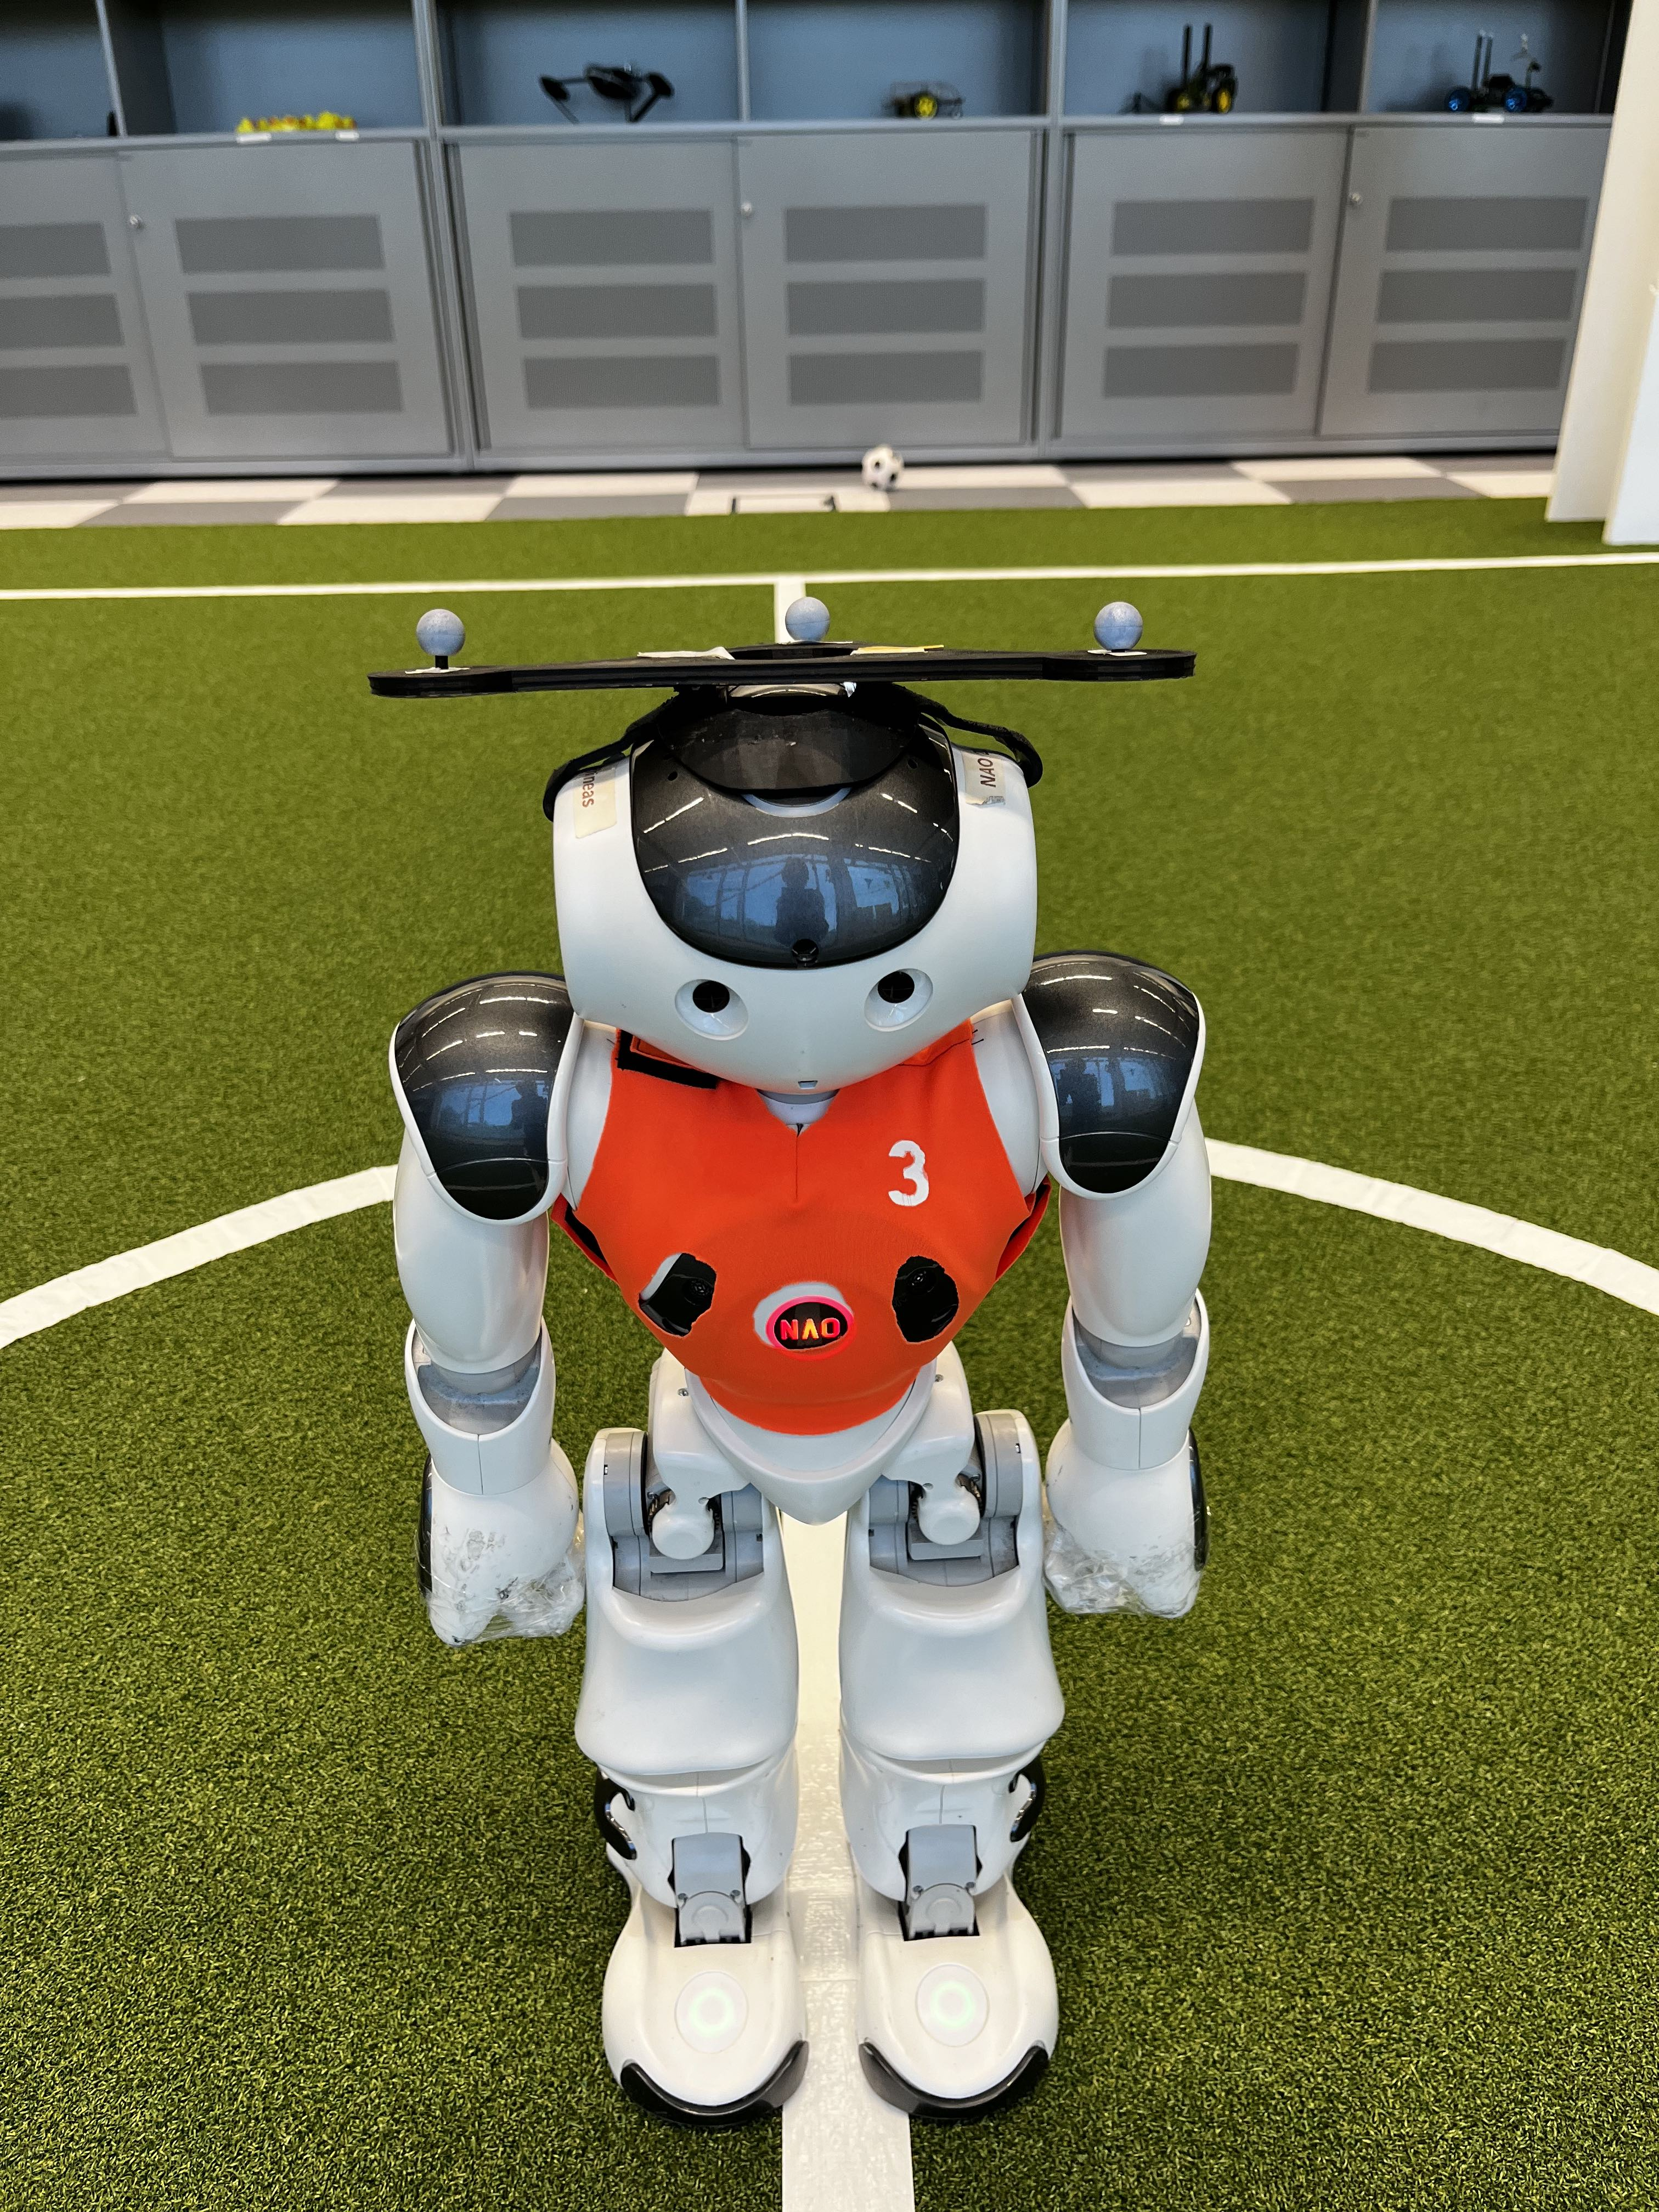
\includegraphics[width=0.34\textwidth]{Scriptie/imgs/optitrackmount.jpg}
            \caption{3D printed Optitrack helmet on the Nao V6 robot.}
            \end{figure}

            In order to verify that a model, which has been trained on virtually generated data, can perform well on real-world inputs, a real-world dataset must first be generated. This was done using the Optitrack system of the Intelligent Robotics Laboratory. This Optitrack system uses eight infrared cameras that track the 3D position of three highly reflective balls, called markers. Figure 3.5 depicts the mounting mechanism that was used to attach the markers to the robot. This mechanism neatly clips on to the robot's head and was designed and 3D-printed by Nuno Scholten, a member of the Dutch Nao Team. The Optitrack system was first calibrated to achieve a mean 3D error of 0.397 millimetres, which the system itself classifies as \textit{exceptional}.
            
            In order to avoid false-positive detections of markers in the recorded position data, a rigid body is constructed from the three markers that are on the robot's head. After the Optitrack data has been recorded, the option to only export rigid body data is used. 

            \begin{figure}[H]
            \centering
            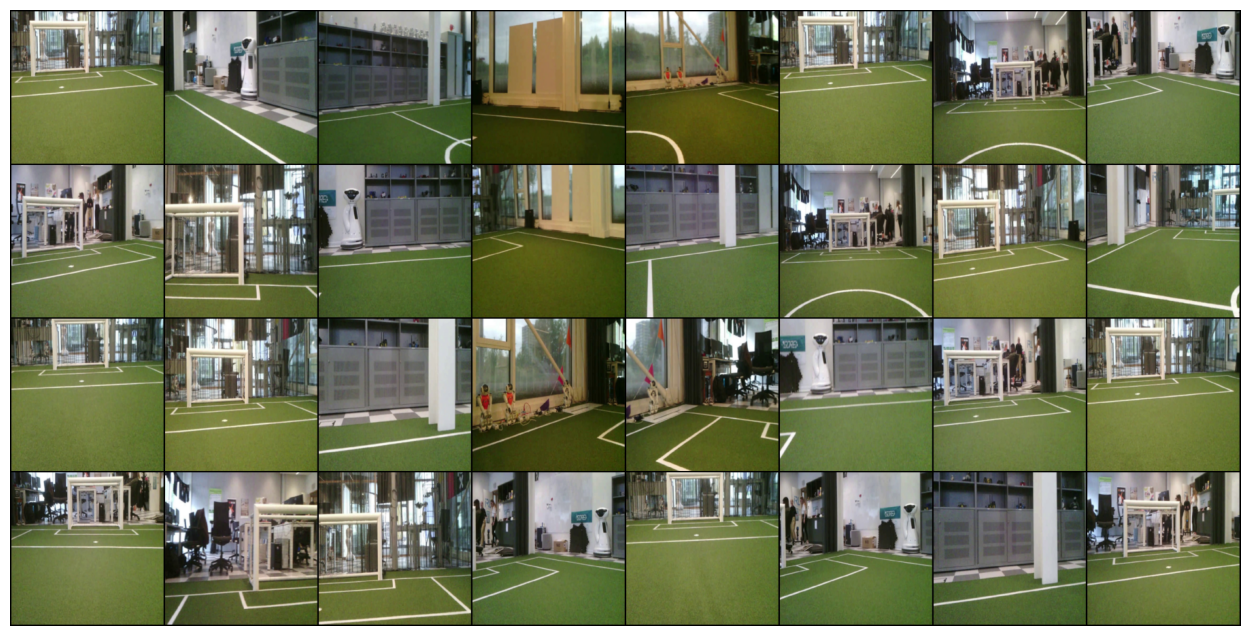
\includegraphics[width=0.85\textwidth]{Scriptie/imgs/real_world2.png}
            \caption{32 example images of the dataset recorded with the Nao V6's cameras.}
            \end{figure}

            Figure 3.6 shows a subset of the images the robot's camera captured of the real-world football field. In total, 4231 samples were taken. The images taken by the robot's camera were synced to the data captured by the Optritrack system based on timestamps.
            As visible in the example images of Figure 3.6, the lighting conditions can differ between separate images, even when those images are recorded at the same time of day. 

\chapter{Experiments}
    This chapter will discuss the performance of the trained model. First, the performance of the model on the virtual dataset is discussed, followed by the performance of the model on the real-world verification dataset.
    \section{Virtually generated dataset}
        \begin{figure}[H]
        \centering
        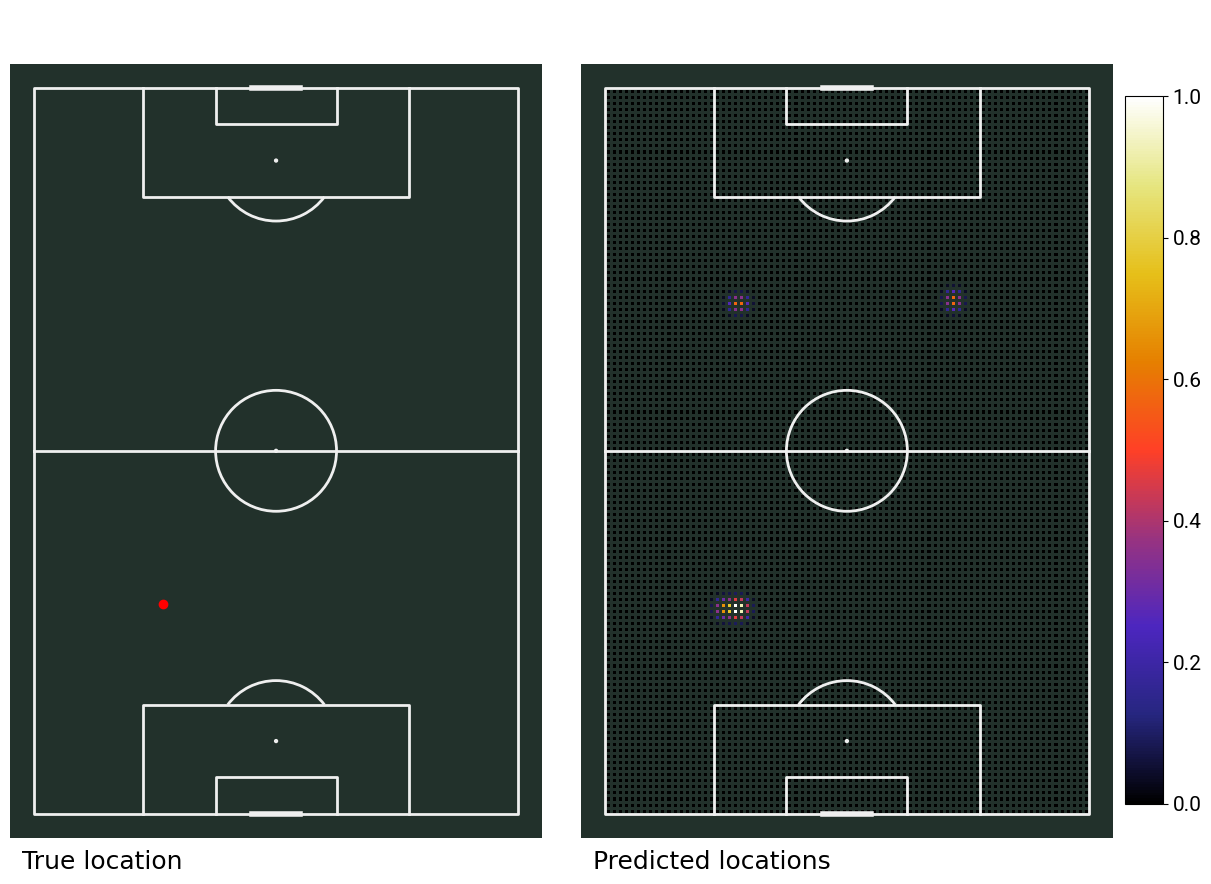
\includegraphics[width=0.95\textwidth]{Scriptie/imgs/sympred.png}
        \caption{True location next to the 10 most confident predictions of the model trained on 225.000 images with 50 epochs. The image that was used to determine the position came from a completely separate virtually generated dataset.}
        \end{figure}

    Figure 4.1 depicts the true location of an input image next to the model's ten most confident guesses. As expected, the guesses are somewhat symmetrical across the football field, except for the bottom right corner. This is expected, as the features of a football field are symmetrical across the centre line. However, because the input image most likely contains features about the environment it was taken in, the model is likely able to correctly predict the location based on these features. A model that would be exclusively trained on data that contains no environmental features would predict the location to be exactly symmetrical. 
    \hfill \break \\
    In order to better quantify the model's performance, the average distance between a predicted position and the true position will be investigated. This way, a classification can still be counted as adequate if it does not differ greatly from the ground truth. If the model were to make completely random guesses, the expected average distance would be 45.92 between the true position and the predicted position, as given by Equation 4.1 with the inputs of (90, 60). Equation 4.1, as proposed in \cite{avgdistance}, gives the average expected distance between two random points on a rectangle. 
    \begin{equation}
    d(a, b) = \frac{1}{15} \left(\left( \frac{a^3}{b^2} + \frac{b^3}{a^2}\right) + \sqrt{a^2 + b^2} \left(3 - \frac{a^2}{b^2} + \frac{b^2}{a^2}\right)\right) + \frac{1}{6}\left(\frac{b^2}{a} ln\left(\frac{a + \sqrt{a^2 + b^2}}{b}\right) + \frac{a^2}{b}ln\left(\frac{b + \sqrt{a^2 + b^2}}{a}\right)\right)
    \end{equation}

    Evaluating the model on a separate virtually generated dataset with 5000 samples gives an average distance between the most confident predicted location and the true location of \textbf{0.651}. This equates to a real-world difference of 6.51 centimetres.\todo{I am working to extend the notebook that calculates this metric to also include a weighted average of the N most confident predictions.} 

    \section{Real-world dataset}
        \begin{figure}[H]
        \centering
        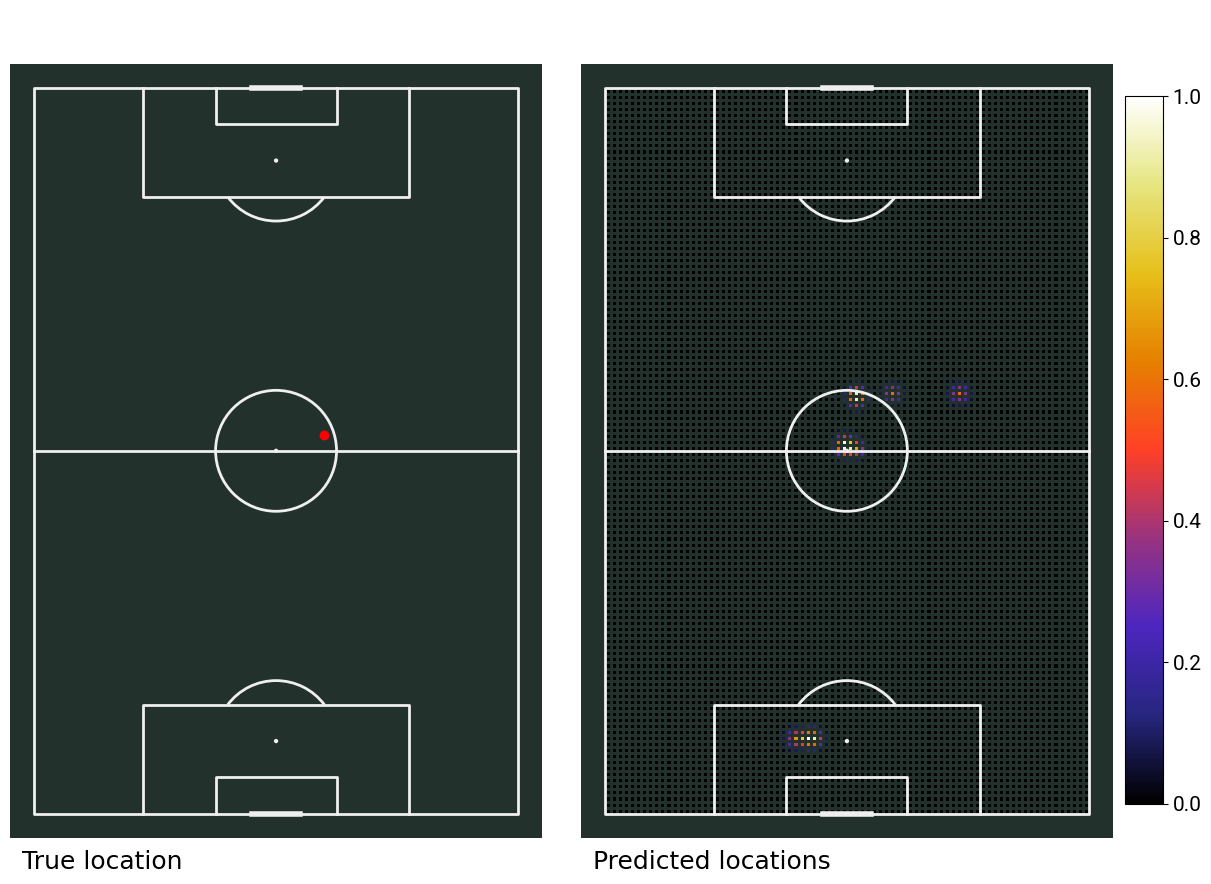
\includegraphics[width=0.95\textwidth]{Scriptie/realexample.png}
        \caption{True location next to the 10 most confident predictions of the model trained on 225.000 images with 50 epochs. The image that was used as input came from the real-world dataset recorded with Optitrack.}
        \end{figure}

        \begin{figure}[H]
        \centering
        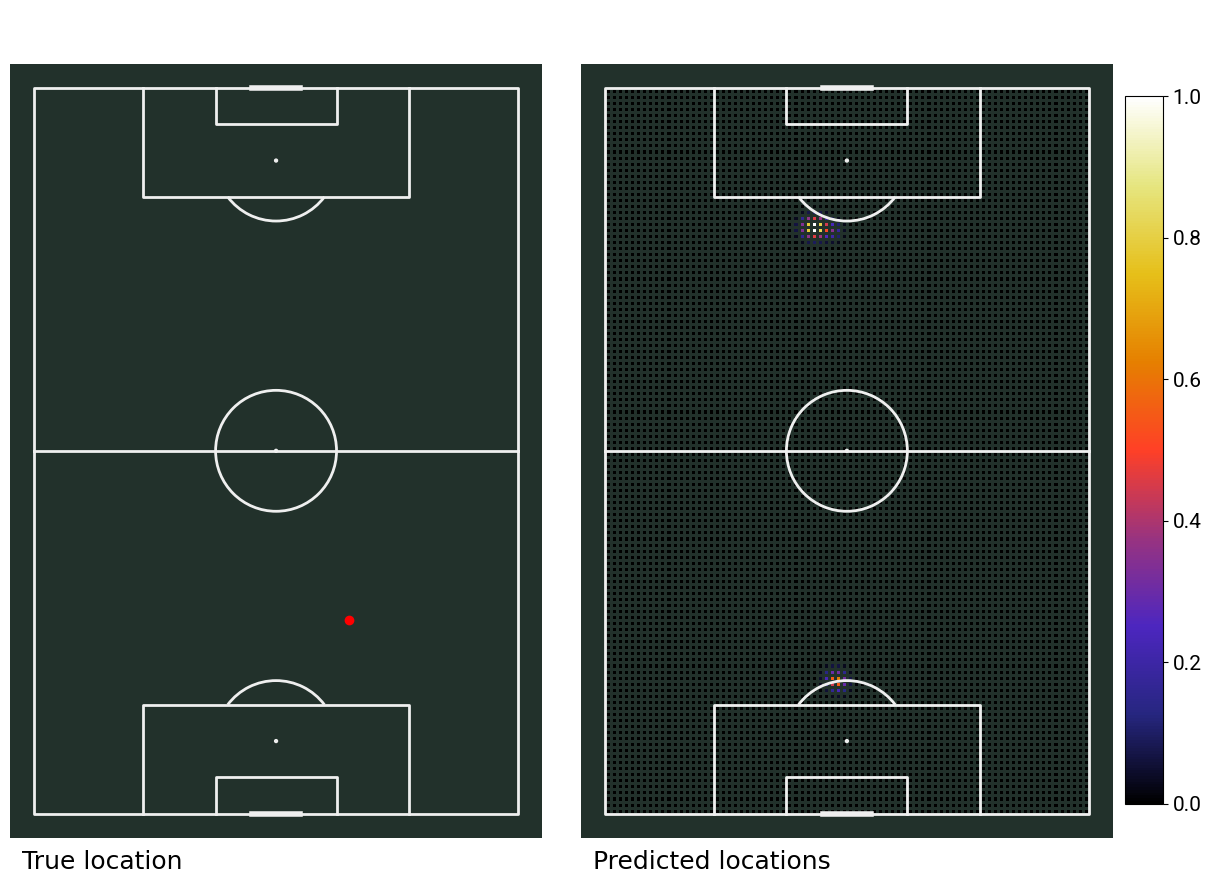
\includegraphics[width=0.95\textwidth]{Scriptie/imgs/real2.png}
        \caption{True location next to the 10 most confident predictions of the model trained on 225.000 images with 50 epochs. The image that was used as input came from the real-world dataset recorded with Optitrack.}
        \end{figure}

        Figure 4.2 and 4.3 show two examples of the model predicting the location from an image in the real-world dataset. The predictions in these two examples have a more significant deviation from the ground truth than the example in Figure 4.1. Calculating the average distance confirms this, as the average distance between the most confident prediction and the true prediction of the real-world verification dataset is \textbf{21.554}. However, the model does show signs of recognising features of the football field. Most predictions in Figure 4.2 are around the centre dot or the penalty dot. In Figure 4.3, all predictions are around the penalty arcs. Based upon the true position in Figure 4.3, it is understandable that these arcs are within view of the robot's camera. 

\chapter{Conclusions}
    % This chapter will discuss the conclusions that can be drawn from the results of the experiments detailed in Chapter 4. This chapter also includes a discussion, in which shortcomings and improvements to this thesis are discussed, as well as a section that highlights possible topics for future research. To conclude, this chapter will end with a section that discusses the ethical remarks of this thesis.
    
    This chapter will discuss the conclusions that can be drawn from the results of the experiments detailed in Chapter 4. This chapter also includes a discussion, in which shortcomings and improvements to this thesis are discussed. This discussion also highlights possible topics for future research. To conclude, this chapter will end with a section that discusses the ethical remarks of this thesis.
    
    \section{Conclusion}
        The results in Section 4.1 and 4.2 show that there is still a significant discrepancy between the model's ability to predict a position on artificially generated dataset compared to real-world dataset.
        The model trained on 225.000 samples achieved an accuracy of 71\% on the virtually generated validation set, with an average distance between the true location and the most confident prediction of \textbf{0.651}. This is within the bounds of a single grid on the football field. However, when the same model is evaluated on a real-world dataset, the average distance between the true position and the best prediction increases to \textbf{21.554}. This indicates that the virtually generated dataset did not manage to successfully bridge the reality gap. However, the results do show that training a machine learning model with virtually generated data is a potentially valid strategy. The virtual environment was able to generate a dataset of a size multiple magnitudes larger than the real-world verification dataset in less time than it took to manually record the dataset. Furthermore, the model does show signs that it is able to pick up on features that it learned from the virtually generated dataset on inputs from the real-world dataset, as well as performing more than twice as well as to when the model were to make completely random guesses. By making several improvements, as detailed in Section 5.2, the gap between the performance on the virtual data and the real-world data could be decreased.

    \section{Discussion}
        \subsection{Image classification problem}
            This thesis proposes a method of dividing the football field into a series of grids, in order to transform the problem of localising the robot into an image classification problem. Therefore, this method defines a specific resolution at which a robot can be localised. As this thesis uses a resolution of 1 decimeter, every classification has a minimum error of 1 decimeter. Furthermore, any space between the grids on the football field does not exist with this method. \\
            There are other possible neural network types that can be explored than the image classification type of GoogLeNet that do not require the football field to be dissected into grids. Instead of having a fully connected neural network that maps to every possible classification in the output layer, the architecture could be transformed into having only two neurons in the output layer that correspond to the predicted x and y coordinate.
            
        \subsection{Bird's-eye view}
            As discussed in this paper, a bird's eye view model would be beneficial to the task of predicting a robot's position on a football field. It was decided that the implementation of the Lift-Splat-Shoot algorithm for this thesis would not be explored further as it took too much time and was blocking other aspects of the research to be explored further. Therefore, the results of this thesis are partially incomplete, as the results are too dependant on the environment of the Intelligent Robotics Laboratory. Furthermore, a correct implementation of a bird's-eye view model could decrease the gap between the artificial and real-world data, because the model can focus more on picking up features from the football field. \\
            In order to generalise the results in the context of football fields at other venues, either a bird's-eye view model must be implemented or a detailed 3D environment of the football field in question must be made accessible in advance. The former provides a more general solution to the problem of determining a robot's position on the football field, and benefits from the positive aspect of virtually generated datasets, namely the cost and time effectiveness of training a machine learning model on virtually generated data.  
            \hfill \break \\
            The Lift-Splat-Shoot algorithm was not the only bird's-eye view model that was explored as a possible implementation for this thesis. It was discussed in more detail in this thesis because it is the state of the art method that is independent on the amount of input channels. Monocular bird's-eye view models were also explored, such as Saha et al. \cite{tomaps} and Li et al. \cite{bimap}. However, these also proved difficult to implement in the context of a NAO V6 robot.

        \subsection{Filtering detections}
            The task of the network used in this paper is to predict the most likely position of an image on a football field. An intuitive approach would be to take the prediction with the highest confidence and interpret that as the robot's current location. However, sometimes the most confident prediction is not the correct position of the robot, as the football field is symmetrical.
            If the localisation method proposed in this thesis were to be implemented on an actual robot, the implementation could take advantage of the odometry system of the robot to make more accurate predictions. Predictions that suddenly appear at a distance far away, further than the robot could possibly travel in the time between the last prediction, could be filtered out. Furthermore, this method gives a suggestion as to which of the most confident predictions is actually correct, as odometry data could be taken into account when extracting the correct prediction from the target vector of the model. \\
            This thesis focused on predicting the location of a single image. However, this is not representative to the real world. In the real world, the input of the localisation algorithm would be a video stream of images. This means that the current position of the robot must logically follow the previous predictions. By implementing memory segments in the neural network, or by implementing a recurrent neural network architecture, the results of a previous prediction can be used to assist the new prediction. 

    % \section{Future work}
    %     \section{Using a bird's-eye view model to }
    %     % As mentioned in section 2.4, the height map that a bird's-eye-view perspective generates can potentially be used to improve the path-finding algorithm of the Dutch Nao Team.

    \section{Ethical remark}
        No data used to train the model for this thesis contains personal information. The only parameters that the model trained on were RGB images, which all contained no recognisable images of people, and the location data the image was taken at. The results of this thesis can also not be used in ways that require specific ethical review, as the method and results of this paper solely focus on determining a robot's position on a football field. This goal of predicting the position of a robot on a football field can not cause harm to people, their privacy nor the environment. 

% \appendix 

\printbibliography

\appendix
\chapter{Appendix}
\newpage
\section{GoogLeNet architecture}
\begin{figure}[H]
\centering
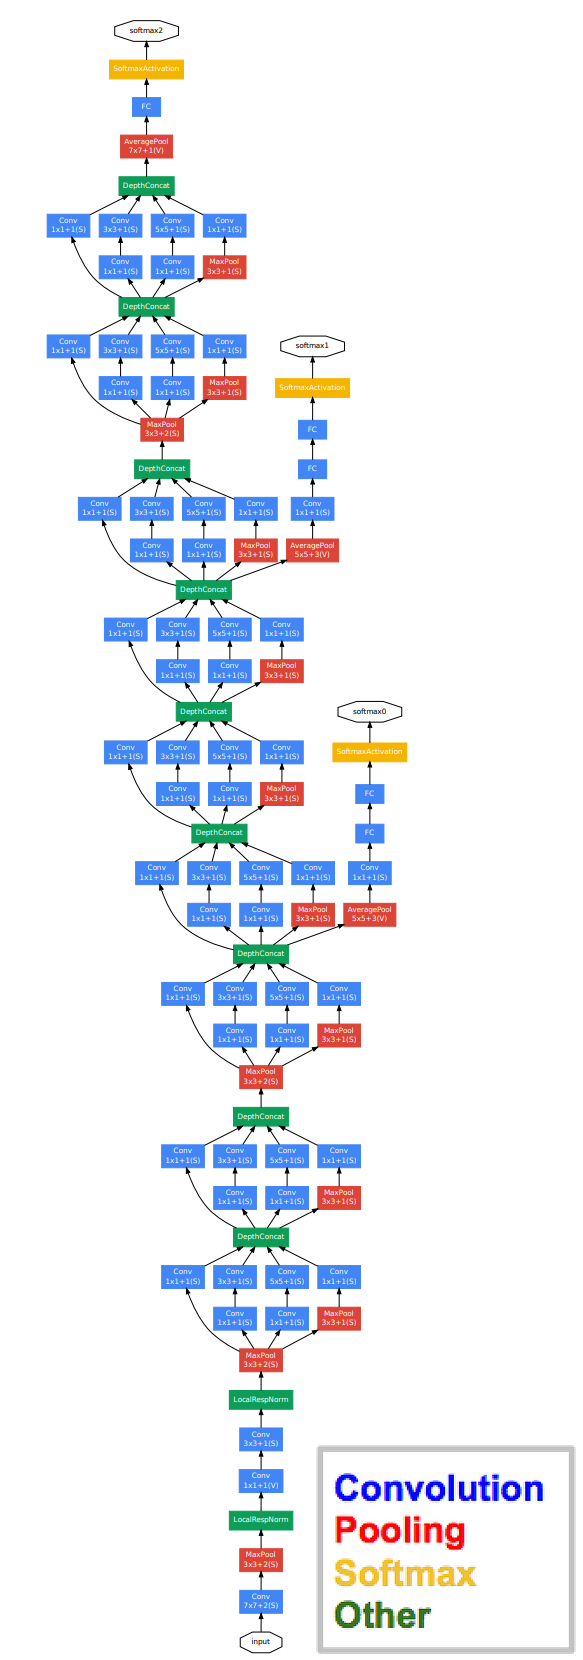
\includegraphics[width=0.55\textwidth]{Scriptie/imgs/googlenetarch.png}
\caption{Architecture of the GoogLeNet convolutional neural network with all of its branches. The architecture depicted is the same as the architecture used to gather the results of this paper. Note: the input layer is at the bottom of the image.}
\end{figure}


\end{document}
